\chapter{Lazart}
\label{chpt:lazart}

\begin{tikzpicture}[remember picture,overlay]
\node[anchor=west,inner sep=0pt] at (current page text area.west|-0,3cm) {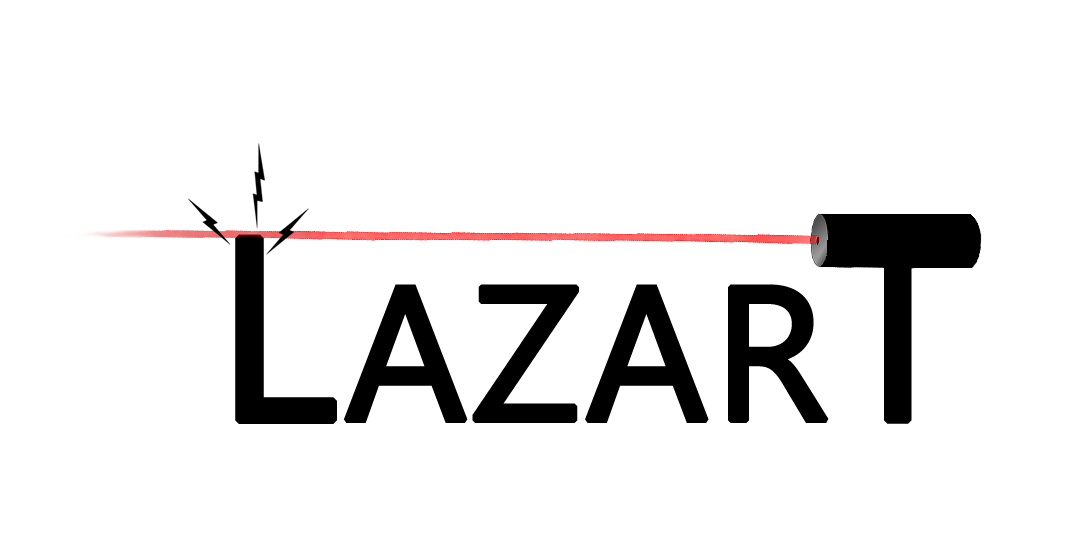
\includegraphics[height=3cm]{ch3-lazart/img/lazart-logo-red.png}};
\end{tikzpicture}

    Lazart \cite{Potet/ICST14} est un outil d'analyse de code haut niveau qui repose sur l'exécution symbolique et vise à évaluer la robustesse d'un programme dans le cadre de l'injection de fautes multiples. 
    Cet outil a été développé à Verimag depuis 2014 et a été étendu au cours de cette thèse. 
    Ce chapitre présente l'outil Lazart, dans sa version la plus récente, en décrivant son fonctionnement et son architecture du point de vue de l'utilisateur. 
    Il s'agira aussi de discuter de ses avantages et limitations par rapport aux outils présentés dans le chapitre précédant.
    Le chapitre \ref{chpt:lazart-implem} rentrera plus en détails dans l'implémentation de Lazart et discutera des choix qui ont été faits pour l'outil.
    
    La suite de ce chapitre est organisée comme suit.  
    La section \ref{sec:lazart-overview} présente le principe général de l'outil, la plateforme \gls{llvm} et l'exécution concolique sur lesquels Lazart s'appuie.
    La section \ref{sec:lazart-architecture} décrit l'architecture de l'outil et les différentes étapes d'une analyse.
    La section \ref{sec:lazart:descr} présente la façon dont l'utilisateur décrit les paramètres d'une analyse avec Lazart.
    La section \ref{sec:lazart-formal} s'intéresse à la représentation des traces dans Lazart ainsi qu'aux analyses de robustesse proposées par l'outil.
    La section \ref{lazart:metho} s'intéresse aux résultats fournis par l'outil, leur exploitation et à l'aspect méthodologique en présentant des évaluations réalisées avec Lazart.
    Finalement, la section \ref{sec:lazart:metho:concl} conclut ce chapitre.
    
    \setcounter{tocdepth}{2}
    \section*{Table des Matières}
    \localtableofcontents
    
    \section{Principe général et pré-requis}
    \label{sec:lazart-overview}
        
        Lazart est un outil d'analyse de code évaluant la robustesse d'un programme dans le cadre d'injection de fautes multiples. Il travaille au niveau de la représentation intermédiaire \gls{llvm-ir} et repose sur l'exécution concolique \cite{Baldoni/CSUR18} (pour concret-symbolique), qui combine l'exécution symbolique avec l'exécution concrète. 
        Lazart est destiné à être utilisé en amont du processus de développement pour aider le développeur à concevoir un programme sécurisé, ou en aval, en apportant une aide aux auditeurs pour en déterminer les vulnérabilités \cite{inter_cesti}. Il propose plusieurs analyses visant à évaluer la robustesse d'un programme dans le cadre de l'injection de fautes.
        L'outil est également destiné à l'évaluation de contre-mesures, cet aspect de l'outil sera présenté plus en détail dans les chapitre \ref{chpt:placement} et \ref{chpt:ccpo}.
        
        \begin{table}[h]
            \begin{center}
                \begin{tabular}{|l|l|l|l|l|l|}
                \hline
                \rowcolor[HTML]{C0C0C0} 
                Limite de faute                           & 0                         & 1                         & 2                         & 3                          & 4                          \\ \hline
                \cellcolor[HTML]{C0C0C0}Attaques       & \cellcolor[HTML]{9AFF99}0 & \cellcolor[HTML]{FFCCC9}1 & \cellcolor[HTML]{FFCCC9}5 & \cellcolor[HTML]{FFCCC9}10 & \cellcolor[HTML]{FFCCC9}11 \\ \hline
                \rowcolor[HTML]{FFCCC9} 
                \end{tabular}
                \caption{Résultat d'analyse d'attaque sur verify\_pin avec Lazart \label{tbl:vp-results}}
            \end{center}
        \end{table}
        
        L'analyse d'attaque permet de rechercher des chemins d'attaques dans un programme, en fonction d'un modèle d'attaquant (objectif d'attaque et modèle de faute). Cette analyse retourne la liste des chemins d'exécution fautés trouvés pour lesquels l'objectif d'attaque est atteint. La table \ref{tbl:vp-results} correspond aux résultats d'une analyse d'attaque pour le programme \texttt{verify\_pin} avec le modèle de l'inversion de test, une limite de fautes de quatre et comme objectif d'attaque $\phi_{auth}$, c'est-à-dire s'authentifier malgré un \gls{pin} faux. Chaque colonne indique le nombre de chemins d'attaques trouvés (deuxième ligne) pour un nombre de fautes fixé (première ligne).
     
        Lazart émule les fautes au niveau de la représentation intermédiaire \gls{llvm} et transmet le programme muté à l'exécution concolique de manière à explorer tous les chemins avec toutes les combinaisons de fautes possibles.
        La section \ref{sec:llvm} présente la plateforme \gls{llvm} et la représentation intermédiaire \gls{llvm-ir}, niveau auquel sont représentées les fautes.
        La section \ref{sec:se} présente le fonctionnement de l'exécution symbolique et la section \ref{sec:dse} décrit l'exécution concolique et les problématiques liées à ce mode de génération de traces. La section \ref{sec:klee} présente plus en détail l'outil KLEE et ses fonctionnalités et finalement, la section \ref{sec:dse-fi} s'intéresse à la façon dont les fautes sont simulées dans une implémentation pour le moteur d'exécution symbolique.
        
        \subsection{Low Level Virtual Machine (LLVM)}
        \label{sec:llvm}
        
            Lazart repose sur la plateforme \gls{llvm} \cite{llvm}, qui est un ensemble d'outils pour la conception de compilateurs, d'optimiseurs et d'outils d'analyse statique. \gls{llvm} est destiné à faciliter l'analyse et l'optimisation de programmes tout au long de la durée de vie d'un programme (\textit{lifelong program analysis and transformation}).            
            
            L'architecture \gls{llvm} (figure \ref{fig:llvm-arch}) s'organise autour de trois blocs majeurs: le front-end, la représentation intermédiaire et le back-end. 
            
            \begin{figure}[!h]\centering
                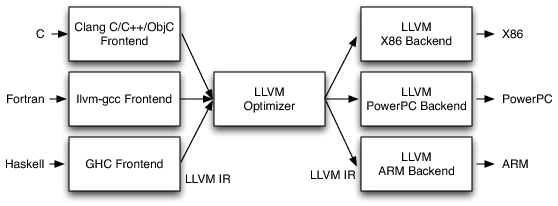
\includegraphics[scale=0.6]{ch3-lazart/img/LLVMCompiler.png}
                \caption{Architecture d'un compilateur en trois temps \cite{llvm/TAOSA}}  \label{fig:llvm-arch}
            \end{figure}
            
            Le \textit{front-end} compile le code source du programme en la \textit{représentation intermédiaire} qui est transformée en code binaire spécifique à l'architecture cible par le \textit{back-end}. Clang \cite{llvm} est certainement le front-end de compilateur le plus célèbre de \gls{llvm} et permet la compilation des langages C, C++, Objective-C et Objective-C++. \gls{llvm} supporte d'autres langages, tels que Rust, Swift, Haskell, D et Ada pour n'en citer que quelques uns, au travers d'autres front-end.
            
            Les analyses et optimisations sont effectuées sur la représentation intermédiaire \gls{llvm-ir}. La figure \ref{fig:llvm-arch} présente le cycle de vie d'un programme dans le cadre d'une compilation \gls{aot}, c'est-à-dire lorsque le processus d'optimisation et d'analyse a lieu en amont de l'exécution du programme. L'architecture de \gls{llvm} permet de simplifier l'optimisation inter-procédurale (\textit{link-time optimization}) en gardant la même représentation intermédiaire tout au long du cycle de vie. \gls{llvm} prend aussi en charge d'autres cycles de vie de programmes tels que:
            
            \begin{itemize}
                \item \textit{Install Time Optimisation}: le programme est optimisé au moment de son installation sur l'appareil. Il s'agit d'un type particulier de compilation \gls{aot} \footnote{C'est par exemple la méthode employée sur Android avec la machine virtuelle Dalvik (qui n'est pas basée sur \gls{llvm}).} qui permet d'avoir des informations exactes sur l'architecture et la machine cible.
                \item \gls{jit} optimisation : le programme est compilé et optimisé pendant son exécution. Le \gls{jit} est très largement utilisé pour les langages basés sur une machine virtuelle (Java, C\# par exemple).
                \item \textit{Idle Time Optimisation}: le programme peut-être optimisé entre les exécutions. 
            \end{itemize}            
            
            \paragraph{}
            La représentation intermédiaire de \gls{llvm} est ainsi manipulée par des passes d'analyse et d'optimisation tout au long de la durée de vie du programme. \gls{llvm-ir} est un langage correspondant à une abstraction des langages assembleur. Sa forme binaire (utilisée en mémoire pendant les opérations ou stockée sous la forme de fichier) peut être transformée en équivalent textuel (et inversement). Le listing \ref{lst:llvm} présente un exemple de code \texttt{Hello world} en \gls{llvm-ir} sous forme textuelle. 
        
\begin{center}
\lstset{language=C,style=codeC} 
\begin{lstlisting}[caption=Programme \textit{Hello World!} en IR LLVM (LLVM-9), label=lst:llvm]
@.str = private unnamed_addr constant [14 x i8] c"Hello world !\00", align 1

define dso_local i32 @main(i32 %0, i8** %1) {
  %3 = alloca i32, align 4
  %4 = alloca i32, align 4
  %5 = alloca i8**, align 8
  store i32 0, i32* %3, align 4
  store i32 %0, i32* %4, align 4
  store i8** %1, i8*** %5, align 8
  %6 = call i32 (i8*, ...) @printf(i8* getelementptr inbounds ([14 x i8], [14 x i8]* @.str, i64 0, i64 0))
  ret i32 0
}

declare dso_local i32 @printf(i8*, ...)
\end{lstlisting}
\end{center}

            \gls{llvm-ir} rend explicite le flot de contrôle et de données. Toute instruction appartient à un bloc de base et tout bloc de base appartient à une fonction. Le langage suit la forme \gls{ssa} \cite{ssa} \footnote{L'instruction \texttt{phi} correspondant à la forme standard (non-gated, c'est-à-dire que l'assignation conditionnelle n'est évaluée qu'à partir d'une variable) de la fonction $\phi$ de \gls{ssa}.} 
            qui impose que chaque variable soit assignée avant toute utilisation et que chaque variable soit assignée exactement une fois. \gls{llvm-ir} utilise un nombre infini de registres typés, identifiés par les $\%XX$ dans le programme d'exemple.
            Les conventions d'appels de fonctions sont abstraites à l'aide des instructions \texttt{ret} et \texttt{call}.
            
            Le langage utilise un jeu d'instructions comparable à \gls{risc} et est fortement typé. Toutes les conversions sont explicites, à l'aide notamment des instructions de conversion (\texttt{cast}, \texttt{trunc}, \texttt{zext} ...) et de l'instruction \texttt{getelementptr} qui permet d'abstraire les opérations d'arithmétique de pointeur tout en préservant le typage (c'est-à-dire que \texttt{getelementptr} effectue les calculs appropriés au type sous-jacent des opérandes). La ligne 10 du programme \ref{lst:llvm}  correspond à l'appel de la fonction C standard \texttt{printf} et l'accès à la chaîne de caractère globale \texttt{@.str} utilise l'instruction \texttt{getelementptr} \footnote{le mot clef \texttt{inbound} est utilisé (ligne 10) pour apporter des garanties sur l'accès à la mémoire pour les phases d'analyse.}.
            
            Les instructions \gls{llvm-ir} peuvent être utilisées de façon générique pour chaque type de donnée de base et existent en plusieurs versions. Par exemple, l'instruction arithmétique \texttt{add} est la même pour les différents types entiers ou flottant et supporte différentes opérandes (par exemple deux registres \texttt{add i16 \%var1, \%var2} ou bien avec une valeur immédiate \texttt{add i64 \%var, i64 10}).            
            
            L'allocation de mémoire fait la distinction entre la pile et le tas. Dans l'exemple \textit{Hello world} ci-dessus, une instruction \texttt{alloca} est utilisée pour allouer un espace mémoire sur la pile pour chaque argument et variable locale de la fonction \texttt{main} (\texttt{\%3}, \texttt{\%4} et \texttt{\%5}). L'allocation sur le tas est effectuée avec l'appel des primitives (par exemple \texttt{malloc} et \texttt{free}). La lecture et l'écriture en mémoire sont faites respectivement avec les instructions \texttt{load} et \texttt{store}. Dans l'exemple \ref{lst:llvm}, chaque opération précise l'alignement des données avec le mot clef \texttt{align}.
            
            La plateforme \gls{llvm} est largement utilisée dans le monde de la recherche et de l'industrie et la page \gls{llvm} \cite{llvm/pub} recense plus de 250 publications liées à la plateforme. Le projet \gls{llvm} sur Github \cite{llvm/github} compte plus de 4000 forks et 2000 contributeurs.  
     
        \subsection{Principe de l'exécution symbolique}
        \label{sec:se}
            
            L'exécution symbolique est une technique d'analyse de programme qui a été théorisée dans les années 70 \cite{Boyer/ACM75, King/ACM76, Clarke/TSE76} et qui vise à générer des entrées de tests pour couvrir chaque partie d'un programme. Le principe consiste à parcourir le programme en utilisant des \textit{variables symboliques} plutôt que des valeurs concrètes pour les entrées, et de résoudre la formule logique associée à chaque chemin d'exécution. 
            L'exécution \textit{dynamique-symbolique} regroupe un ensemble de techniques se basant sur une combinaison d'une exécution symbolique et d'exécution(s) concrète(s) dans le but d'adresser certaines problématiques liées à l'exécution symbolique (section \ref{sec:dse}).
            
            Pour la fonction \texttt{exemple} en Figure \ref{lst:dse-example}, un chemin d'exécution possible consiste à passer dans la branche \textit{then} de la première condition et atteindre l'assertion dans la branche \texttt{else} ligne 9. Un ensemble d'entrées possible pour arriver à cet état est $\{x = 1, y = 3\}$. On peut alors chercher s'il existe un ensemble d'entrées invalidant l'assertion, comme par exemple $\{x = 0, y = 3\}$. L'objectif d'un outil d'exécution symbolique est d'obtenir une couverture maximale des chemins du programme et de fournir des valeurs concrètes pour les entrées permettant d'exécuter chaque chemin.
   
            \begin{center}
            \lstset{language=C,style=codeC}    
            \begin{lstlisting}[caption=La fonction exemple, label=lst:dse-example]
void exemple(int x, int y) { 
    if (x + y > 2) {          
        z = 2*x + y;              
        if (z == 20) {       
            x = y;        
            print(x);          
        }
        else {         
            y *= 2;      
            assert(x != 0);
        }
    }
    else {                  
        foo();             
    }
}
            \end{lstlisting}
            \end{center}    
                
            Le moteur d'exécution symbolique maintient un \textit{état symbolique} et un \textit{prédicat de chemin}.
            L'\textit{état symbolique} $\sigma$ associe aux variables une expression symbolique qui est mise à jour à chaque fois qu'une affectation est rencontrée. Pour une affectation $var = expr$, $\sigma$ est mis à jour en associant $var$ à $\sigma(expr)$. La figure \ref{lst:dse-example-sigma} présente le code de la fonction \textit{exemple} avec l'évolution de l'état symbolique à chaque assignation dans le programme.
            
            \begin{center}
            \lstset{basicstyle=\large}
            \lstset{language=C,style=codeC}    
            \begin{lstlisting}[caption=Etats symboliques pour la fonction exemple, escapeinside={(*}{*)}, label=lst:dse-example-sigma]
void exemple(int x, int y) {    (* {\color{red} $\sigma \: = \: \{ \: x \: \to x_0, \: y \: \to \: y_0  \: \} $}*)
    if (x + y > 2) {        
        z = 2*x + y;            (* {\color{red} $\sigma \: = \: \{ \: z \: \to \: 2*x_0 \: + \: y_0, \: x \: \to x_0, \: y \: \to \: y_0 \: \} $}*)
        if (z == 20) {       
            x = z + 3;          (* {\color{red} $\sigma \: = \: \{ \: z \: \to \: 2*x_0 \: + \: y_0, \: x \: \to 2*x_0 \: + \: y_0 + \: 3, \: y \: \to \: y_0 \: \} $}*)
            print(x);           
        }
        else {
            y *= 2;             (* {\color{red} $\sigma \: = \: \{ \: z \: \to \: 2*x_0 \: + \: y_0, \: x \: \to x_0, \: y \: \to \: 2 * y_0 \: \} $}*)
            assert(x != 0);
        }
    }
    else {
        foo();      
    }
}
            \end{lstlisting}
            \end{center}     
         
            Le \textit{prédicat de chemin} (\gls{pathc}) est une formule logique du premier ordre qui est mise à jour à chaque fois qu'un branchement conditionnel est rencontré.
            La fonction \textit{exemple} contient donc cinq prédicats de chemin, présentés dans le listing \ref{lst:dse-example-pc}, dont les valeurs sont:
            
            \begin{eqnarray}
                PC_0 & \equiv & true \\
                PC_1 & \equiv & x_0 + y_0 > 2 \\
                PC_2 & \equiv & x_0 + y_0 > 2 \wedge 2 * x_0 + y_0 = 20 \\
                PC_3 & \equiv & x_0 + y_0 > 2 \wedge 2 * x_0 + y_0 \ne 20 \\
                PC_4 & \equiv & x_0 + y_0 <= 2 
            \end{eqnarray}
            
            \begin{center}
            \lstset{basicstyle=\large}
            \lstset{language=C,style=codeC}    
            \begin{lstlisting}[caption=La fonction exemple, label=lst:dse-example-pc]
void exemple(int x, int y) {    // PC0
    if (x + y > 2) {            // PC1
        z = 2*x + y;              
        if (z == 20) {          // PC2
            x = y;        
            print(x);          
        }
        else {                  // PC3
            y *= 2;
            assert(x != 0);  
        }
    }
    else {                      // PC4   
        foo();            
    }
}
            \end{lstlisting}
            \end{center} 
            
            Lorsqu'un branchement $if( expr )$ est rencontré, le prédicat de chemin est mis à jour tel que $PC_{then} = PC \wedge \sigma(expr)$ pour la branche vraie, et $PC_{else} = PC \wedge \neg \sigma(expr)$ pour la branche fausse. S'il existe une solution qui satisfait $PC_{then}$, l'exécution symbolique clone l'état symbolique $\sigma$ et continue avec le prédicat de chemin $PC_{then}$ dans la branche \textit{then}, et respectivement pour la branche \textit{else}.
            
            \paragraph{}            
            La résolution des prédicats de chemins est automatisée avec des solveurs de contraintes. 
            Les solveurs particulièrement utilisés dans ce contexte sont les solveurs \gls{smt} \cite{DeMoura/ACM11, Barrett/HMC18} qui permettent de prouver la satisfaisabilité de certaines classes de formules logiques du premier ordre sans quantificateur. Le solveur de contraintes prend en entrée une formule logique et peut indiquer si elle est satisfaisable (en exhibant une valuation des variables correspondantes), si elle est non satisfaisable (il n'existe aucune solution), ou bien ne pas conclure dans le temps imparti (\textit{timeout}). 
            
            L'évolution des solveurs \gls{smt} au cours de ces dernières décennies a permis de rendre réaliste l'usage des techniques d'exécution symbolique. Parmi les principales théories supportées on trouve l'arithmétique linéaire ou non linéaire (sur entiers ou réels), les tableaux, les vecteurs de bits, etc. 
            
            \paragraph{}            
            \begin{sloppypar}   
            On peut s'intéresser à la correction et la complétude des prédicats de chemins \cite{Godefroid/PLDI11}.
            \end{sloppypar}   
            
            \begin{defi}
            \label{def:pc-sound}
                Un prédicat de chemin $PC_{\omega}$ est \textit{correct} si tout modèle satisfaisant $PC_{\omega}$ fournit des entrées pour une exécution du programme suivant le chemin $\omega$.
            \end{defi}
            
            \begin{defi}
            \label{def:pc-complete}
                Un prédicat de chemin $PC_{\omega}$ est \textit{complet} si toute entrée suivant le chemin $\omega$ est un modèle validant $PC_{\omega}$.
            \end{defi}
        
        \subsection{Exécution dynamique-symbolique (DSE)}
        \label{sec:dse}                
            
            L'exécution \textit{dynamique-symbolique} (\gls{dse}) consiste à combiner l'exécution symbolique avec l'exécution concrète. Cela permet de résoudre en partie certains des problèmes liés à l'exécution symbolique, potentiellement au prix d'une perte de correction et de complétude lorsqu'une partie de l'analyse est concrétisée.
                   
            \begin{sloppypar}  
            Les premières approches sont apparues dans les années 2000 avec notamment le \textit{test concolique} introduit dans l'outil \gls{dart} \cite{Godefroid/PLDI05}. \gls{dart} propose de maintenir un état concret parallèlement à l'état symbolique. Cette approche nécessite des entrées concrètes au démarrage de l'analyse, qui peuvent être générées aléatoirement ou fournies par l'utilisateur. L'état concret associe chaque variable du programme à une valeur et maintient le prédicat de chemin et l'état symbolique de manière à calculer à l'aide du solveur des valeurs concrètes pour chaque chemin. Cette concrétisation permet notamment d'exécuter des fonctions externes à l'aide de valeurs concrètes sans disposer de leur code.        
            \end{sloppypar}  
            
            EXE \cite{Cadar/ACM08} et son successeur KLEE \cite{Cadar/OSDI08} utilisent une approche similaire que les auteurs nomment \textit{execution-generated testing}, proposée initialement en 2005 \cite{Cadar/SPIN05}, qui maintient également un état concret. Si une opération n'implique que des valeurs concrètes, celle-ci est exécutée directement, sinon, l'opération est effectuée symboliquement. 
            
            L'exécution dynamique-symbolique est limitée par un certain nombre de problématiques: la résolution des prédicats de chemin, le nombre de chemins générés, la modélisation du système et l'utilisation de code non disponible (comme une bibliothèque externe). La suite de cette section s'intéresse à ces problématiques et présente certaines approches qui ont été développées pour les pallier.
            
            \subsubsection{Complexité des formules passées au solveurs}
                
                Les solveurs de contraintes sont sensibles au type d'application considéré. Ils peuvent être limités si les théories supportées ne permettent pas (dans un temps raisonnable) de résoudre le prédicat de chemin ou bien si le prédicat de chemin contient des formules qui sont par nature difficiles à résoudre (comme inverser une fonction de hachage cryptographique par exemple). 
                
                Certaines techniques permettent cependant d'atténuer ces difficultés du côté du moteur d'exécution symbolique. Les formules logiques transmises aux solveurs peuvent être simplifiées ou optimisées par différentes techniques: réutilisation des résultats de résolution de contraintes (\textit{incremental solving} \cite{Sen/SIGSOFT05}),
                suppression des contraintes non liées au test qu'on veut valider ou inverser (\textit{irrelevant constraint elimination} \cite{Cadar/OSDI08}), simplification des expressions logiques passées au solveur, comme des simplifications linéaires ou des remplacements par des expressions équivalentes (par exemple transformer une puissance de 2 en un décalage de bit). La \textit{constraint set simplification} \cite{Cadar/ACM13} vise à simplifier les expressions du prédicat de chemin au fur et à mesure de l'exécution lorsque des contraintes plus précises sont rencontrées (par exemple $x_0 < 4 \wedge x_0 = 1 \: \to \:  x_0 = 1$).
                
                Outre la simplification des contraintes, le moteur d'exécution symbolique peut réduire le nombre d'appels au solveur par plusieurs techniques.
                Tout d'abord, le moteur peut continuer l'exploration sur certains chemins tandis que des requêtes sont en attente pour d'autres chemins. C'est par exemple ce que fait EXE qui utilise un serveur responsable de traiter les requêtes demandée par les différentes instantes du moteur d'exploration.
                Certains outils, tels que KLEE et Binsec \cite{Djoudi/CTACAS15, Binsecgithub}, proposent d'utiliser plusieurs solveurs de contraintes. Ceux-ci peuvent être appelés en parallèle ou bien choisis à l'aide d'heuristiques.  
                Des formats standards de requête aux solveurs tels que SMT-LIB \cite{BarFT-SMTLIB} ont été développés pour faciliter l'interchangeabilité des solveurs.
                La réutilisation des contraintes peut être faite en utilisant un cache des contraintes déjà envoyées au solveur: par exemple le \textit{constraint caching} effectuant du hash consing sur les contraintes \cite{Cadar/ACM13}, ou bien le \textit{counter example caching scheme} de KLEE, qui part du principe qu'en général l'ajout de contraintes n'invalide pas les solutions déjà trouvées.
                L'approche décrite dans \cite{yang2012memoized}, appelée \textit{memoized symbolic execution}, encode les préfixes des chemins d'exécution afin de les réutiliser. 
                Green Framework \cite{visser2012green, jia2015enhancing} propose d'aller plus loin en proposant la réutilisation de contraintes entre des programmes et des analyses différentes.
                Dans les cas où les contraintes sont trop complexes pour le solveur, la concrétisation de certaines variables est une solution. Certaines concrétisation peuvent néanmoins faire perdre la complétude.
                
            \subsubsection{Explosion des chemins}
                
                L'exécution symbolique est aussi sensible à \textit{l'explosion des chemins} (\textit{path explosion}). Le nombre de chemins d'exécution d'un programme peut rapidement devenir grand, voir infini (lorsque le programme contient des boucles dépendantes des entrées - que ce soit des boucles directes telles que des \textit{for}/\textit{while}, ou par récursion). S'il n'est pas possible de borner statiquement le nombre d'itérations, alors l'analyse doit se restreindre à une couverture partielle des chemins d'exécution. 
                
                Pour pallier la problématique d'explosion des chemins, plusieurs heuristiques peuvent être mises en place en plus de borner le nombre d'itérations ou la profondeur d'une exécution \cite{Cadar/OSDI08, Goderfoid/NDSS08, schwartz2010all, jamrozik2013generating}. 
                Ces heuristiques visent généralement en priorité la couverture de code (que ce soit au niveau des instructions ou des branches). Celles-ci comptent notamment la sélection aléatoire de chemins \cite{Cadar/ACM13}, le choix du chemin se rapprochant le plus d'une instruction non couverte, la sélection du chemin le plus court (\textit{shortest distance symbolic execution (SDSE)} \cite{chipounov2012s2e}) ou la sélection des chemins couverts le moins de fois. Certaines stratégies peuvent combiner plusieurs heuristiques (comme \textit{cov new} de KLEE) ou utiliser d'autres techniques comme le fuzzing \cite{majumdar2007hybrid, stephens2016driller, yun2018qsym}.
                
                La combinaison avec d'autres méthodes d'analyse peut également aider dans la réduction du nombre de chemins à explorer. Certaines fonctions peuvent être analysées indépendamment, de manière à générer des pré-conditions et post-conditions sur les entrées et sorties afin d'être ensuite réutilisées lors de l'appel de ces fonctions \cite{Godefroid/PLDI11}.
                Triton \cite{salwanthesis} propose aussi une option pour ne rendre symbolique que les espaces mémoires associés à une valeur teintée, la teinte étant propagée pendant l'exécution à partir des teintes initiales spécifiées par l'utilisateur.

            \subsubsection{Modélisation de l'architecture}
            
                La modélisation de l'architecture cible est également un problème important dans le cadre de l'exécution concolique et de l'analyse statique plus généralement. 
                Un modèle plus précis permet des résultats plus représentatifs mais peut être plus coûteux (notamment à cause d'une plus grande complexité des formules logiques passées aux solveurs). 
                
                Concernant la mémoire, différentes approchent existent. Certains outils considèrent toutes les variables d'un programme comme symboliques par défaut, comme c'est le cas pour Angr \cite{Shoshitaishvili/SSP16} par exemple. 
                D'autres comme KLEE nécessitent que l'utilisateur spécifie quelles sont les variables à rendre symboliques.
                La gestion de KLEE utilise un modèle mémoire composé de \og blocs mémoires \fg{} qui sont des tableaux de vecteurs de bits mais toutes les adresses (pointeurs) sont concrètes \cite{cadar2020klee}. 
                \gls{dart} utilise une approche similaire et concrétise un pointeur en prenant en compte le cas nul et le cas d'un objet complet. 
                Binsec représente la mémoire comme un tableau symbolique \cite{Djoudi/CTACAS15}.
                
                La prise en compte d'un environnement d'exécution complet (appels systèmes, bibliothèques externes, réseau...) est aussi une difficulté importante pour l'analyse statique d'un programme.
                Une solution consiste à interagir avec un environnement réel en concrétisant les paramètres au moment de l'appel. Cette approche est utilisée par EXE, \gls{dart} et CUTE par exemple, mais celle-ci souffre de l'incomplétude de la concrétisation.
                L'interaction avec un environnement concret nécessite de prendre des précautions pour que les interactions d'une exploration de chemin n'aient pas un effet de bord sur un prochain chemin, pour cela des solutions basées sur la virtualisation ont été mises en place (par exemple S2E \cite{chipounov2012s2e} qui utilise QEMU).
                Une autre solution est de rendre symbolique tout retour d'un appel externe afin de prendre en compte tous les comportements, ce qui mène toutefois à une sur-approximation.
                KLEE propose une implémentation de la bibliothèque standard C (appelée $\mu$libc) et qui peut être exécutée concrètement ou symboliquement pendant l'exécution concolique. Klover \cite{li2011klover} supporte aussi des bibliothèques POSIX supplémentaires.
                Certaines approches nécessitent l'intervention de l'utilisateur pour décrire un modèle \cite{xiao2011precise}. 

        \subsection{KLEE}
        \label{sec:klee}
        
            KLEE \cite{Cadar/OSDI08} est l'outil d'exécution symbolique utilisé dans Lazart. C'est un outil \emph{open-source} \cite{Klee/github} basé sur llvm-ir. En plus des caractéristiques déjà évoquées dans les sections précédentes, KLEE propose le paramétrage des stratégies d'exploration des chemins, le choix des solveurs à utiliser et l'accès aux formules \gls{smt} générées. L'outil supporte les solveurs STP \cite{ganesh2007decision}, boolector \cite{brummayer2009boolector}, CVC4 \cite{BarrettCDHJKRT11}, Yices 2  \cite{dutertre2014yices}, Z3  \cite{DeMoura/ACM11} et meta SMT \cite{haedicke2011metasmt}, qui est un projet permettant de supporter plusieurs solveurs de façon générique. 
            
            KLEE a été utilisé pour analyser la bibliothèque COREUTILS \cite{Coreutils} (plus de 400k lignes de code) et a permis de trouver 56 bugs majeurs dont 3 qui étaient inconnus jusqu'alors \cite{Cadar/OSDI08}. 
            L'outil a fini second lors de la compétition TestComp 2019 \cite{cadar2020klee} avec 1226 points contre 1238 pour l'outil Verifuzz \cite{basak2019verifuzz}, en ayant presque aucun point dans la catégorie des nombres en virgule flottante puisque ceux-ci ne sont pas supportés par KLEE.
            
            L'outil est largement utilisé pour différents types d'analyse de code (test fonctionnel, recherche de vulnérabilités, tolérance aux fautes, etc.) et la page \cite{klee-ref} recense plus de 100 publications liées à l'outil.
            Un certain nombre de projets ont été proposés à partir de KLEE.
            Cloud9 \cite{bucur2011parallel} est un projet open-source qui permet d'effectuer de l'exécution symbolique parallélisée avec KLEE, ce qui peut fortement améliorer les performances.
            Klover \cite{li2011klover} est une extension de KLEE proposant un support complet du C++ et qui utilise un solveur spécialisé pour les chaînes de caractères. 
            KleeNet \cite{sasnauskas2010kleenet} est un outil basé sur KLEE visant la recherche de chemins d'erreur dans des systèmes distribués et les piles de protocoles réseaux.
               
            \begin{sloppypar}  
            Le listing \ref{lst:klee} présente un exemple utilisation de KLEE contenant une fonction \texttt{foo} effectuant un branchement et le code d'analyse dans la fonction \texttt{main}.
            La fonction \texttt{klee\_make\_symbolic} (lignes 11 et 12) est utilisée pour déclarer une variable comme symbolique, la fonction prend en paramètre un pointeur vers la zone mémoire à rendre symbolique, sa taille et un nom (utilisé pour l'affichage des résultats).
            La fonction \texttt{klee\_assume} permet de couper l'exploration des chemins qui ne valident pas le prédicat en argument. Dans l'exemple (ligne 16), l'exploration se restreint aux exécutions où le retour de \textit{foo} est strictement positif. Cela permet d'encoder la vérification d'un objectif d'attaque par exemple.
            \end{sloppypar}  
            
            \begin{minipage}{\linewidth}
            \lstset{basicstyle=\large}
            \lstset{language=C,style=codeC}    
            \begin{lstlisting}[caption=Exemple d'instrumentation du programme pour KLEE, label=lst:klee]
int foo(int a, int b)
{
    if(b == 0)
        return a;
    return a / b;
}

int main() {
    int a;
    int b;
    klee_make_symbolic(&a, sizeof(a), "a"); // (memory pointer, size, name)
    klee_make_symbolic(&b, sizeof(b), "b");
    
    int result = foo(a, b);
    
    klee_assume(result > 0); // attack objective.
}
            \end{lstlisting}
            \end{minipage}
                
            KLEE fournit un ensemble de cas de tests (sous la forme de fichiers .ktest) qui correspondent chacun à un représentant d'un prédicat de chemin. Chaque cas de test est aussi associé à un type de terminaison qui peut être notamment:
            \begin{itemize}
                \item Une erreur d'exécution: adresse invalide lors d'une écriture ou lecture mémoire (\textit{ptr}), arithmétiques (division par zéro (\textit{div}), dépassement d'entier (\textit{overflow})), pointeur invalide fournit à \texttt{free} (\textit{free}), violation d'une mémoire read-only (\textit{rom}).
                \item Des comportement spécifiques: arrondi implicite (\textit{trunc}), conversion implicite (\textit{conv}).
                \item Une sortie secondaire: appel à la fonction standard \texttt{abort} ou à \texttt{klee\_abort} (\textit{abort}), assertion invalide (\textit{assert}). 
                \item Une erreur utilisateur (\textit{user}): un assume faux (\texttt{klee\_assume}) ou une utilisation incorrecte de KLEE.
                \item Concrétisation forcée (\textit{model}): appel symbolique à une fonction externe ou allocation de mémoire de taille symbolique par exemple.
                \item Une terminaison normale (aucun \texttt{klee\_assume} n'est violé) (\textit{satisfy}). 
                \item Un timeout: le chemin n'a pas pu être exploré dans le temps imparti (\textit{timeout}). 
            \end{itemize}            
            
            KLEE propose par ailleurs une fonctionnalité de replay qui permet de rejouer une exécution à partir d'un ktest en utilisant les valeurs du représentant pour les variables symboliques. Cela permet d'observer les sorties de l'exécution de ce chemin (sortie console ou interaction avec des fichiers par exemple).
            
        \subsection{Exécution symbolique et injection de fautes}
        \label{sec:dse-fi}
        
            Comme dit au début de ce chapitre, Lazart se base sur l'exécution concolique et le parcours des chemins pour chercher des attaques en fautes multiples. Cette section explique comment les fautes sont émulées pour le moteur d'exécution concolique.
        
            Le déclenchement potentiel d'un point d'injection est représenté à l'aide d'une variable symbolique interprétée comme un booléen, comme présenté dans la figure \ref{fig:symbolic-ip-pc}. Lorsque l'exécution symbolique rencontre un point d'injection, l'exécution est divisée en un chemin non fauté et un chemin fauté. 
            La fonction \texttt{symbolic\_bool} correspond à la génération d'une variable symbolique booléenne et la condition ligne 2 induit une division des chemins.
            Soit $PC_0$ le prédicat de chemin précédant le point d'injection, alors le chemin sans faute a pour prédicat de chemin  $PC_{normal} \equiv PC_0 \; \wedge \; \neg inject$ et celui fauté  $PC_{inject} \equiv PC_0 \; \wedge \; inject$. 
            Dans cet exemple, les variables \textit{\_fault\_count} et \textit{\_fault\_limit} correspondent respectivement au nombre de fautes injectées dans l'exécution en cours et à la limite de fautes.
            C'est en cela que l'approche utilisée par Lazart s'apparente aux outils de type \gls{swifi}, présentés dans le chapitre \ref{chpt:background}.
    
            \begin{figure}[H]\centering
            \begin{multicols}{2}
\lstset{language=C,style=codeC, caption={Comportement nominal},label=lst:symbolic-ip-nominal, showlines=true}
\begin{lstlisting}
normal_behavior()






\end{lstlisting}  
\columnbreak

\lstset{language=C,style=codeC, caption={Comportement avec fautes},label=lst:symbolic-ip-fault}
\begin{lstlisting}[label=lst-symbool]
inject = symbolic_bool()
if inject and _fault_count <= 
        _fault_limit:
    _fault_count++
    faulted_behavior()
else:
    normal_behavior()
\end{lstlisting}  
            \end{multicols}
            \caption{Représentation des fautes en pseudo-code pour l'exécution symbolique \label{fig:symbolic-ip-pc}}
            \end{figure}
        
            Ainsi l'exécution symbolique effectue un parcours de l'arbre d'exécution en y incluant toutes les exécutions fautées possibles. Cette disjonction des cas intensifie le phénomène d'\textit{explosion des chemins}, tout particulièrement dans le cadre de fautes multiples.
            Les fautes peuvent aussi introduire des chemins qui ne terminent pas.
            
            Illustrons cette explosion de chemins avec l'exemple de la fonction \texttt{fib} présentée dans le listing \ref{lst:fib} et qui correspond à une implémentation récursive du calcul de la suite de Fibonacci. Dans une exécution non fautée, cette fonction est constituée d'un ensemble d'exécutions correspondant à l'appel récursif de la fonction \texttt{fib} dépendant de l'entier naturel n.
    
\begin{lstlisting}[caption=Fonction \texttt{fib}, label=lst:fib]
uint fib(uint n) {
    if (n <= 1)
        return n;
    return fib(n-1) + fib(n-2); // IP1 et IP2
}
\end{lstlisting}  

            Si on considère un modèle de faute permettant de remplacer le retour d'un appel à \texttt{fib} par \texttt{0}, le programme contient deux points d'injection à la ligne 4, c'est-à-dire \texttt{fib(n-1)} ($IP_1$) et \texttt{fib(n-2)} ($IP_2$). Cela implique qu'à chaque appel à la fonction \texttt{fib(n)} dans une exécution normale, le chemin d'exécution se divise en cinq: le chemin retournant $n$, le chemin retournant \texttt{fib(n-1) + fib(n-2)} et les trois chemins fautés avec le déclenchement des points d'injection $\{IP_1\}$, $\{IP_2\}$ et $\{IP_1, IP_2\}$.
            
            Pour une exécution avec une valeur d'entrée $n$ fixée, l'exécution non fautée produit un unique chemin dont le nombre de blocs de base traversés dépend de $n$. Pour une exécution fautée, il existe $5^n$ chemins, pour un nombre de fautes non borné. 
            L'explosion du nombre de chemins est donc renforcée par la combinatoire des fautes en particulier en fautes multiples (ce problème est lié à l'injection de fautes et n'est pas spécifique à l'exécution concolique).
            
            \paragraph{}
            
            Les définitions \ref{def:pc-sound} et \ref{def:pc-complete} présentées précédemment définissent la \textit{correction} et la \textit{complétude} d'un prédicat de chemin $PC_{\omega}$.
            Soit $\Omega^M$ l'ensemble des chemins d'exécution fautée pour un programme $P$ et un modèle de faute $M$. 
            Un chemin d'exécution fautée $\omega \in \Omega^M$ peut correspondre à une exécution nominale (sans-faute) ou une attaque (exécution avec au moins une faute).
            On note $\mathcal{E}^M$ l'ensemble des prédicats de chemins fautés produits par un moteur d'exécution symbolique fauté $\epsilon$, séparant l'exploration des chemins entre le cas fauté et le cas non fauté, à chaque fois qu'un point d'injection est rencontré.
            
            On peut alors s'intéresser à la \textit{correction} et la \textit{complétude} d'un prédicat de chemin fauté $PC^M_{\omega}$, qui fournit des entrées et des fautes menant à une exécution suivant le chemin d'exécution fauté $\omega$ (définitions \ref{def:pcf-sound} et \ref{def:pcf-complete}).
            Les définitions \ref{def:fi-sound} et \ref{def:fi-complete} s'intéressent respectivement à la \textit{correction} et la \textit{complétude} de l'énumération des prédicats de chemins fautés $\mathcal{E}^M$ par un moteur d'exécution symbolique fauté $\epsilon$.
            
            \begin{defi}
            \label{def:pcf-sound}
                Un prédicat de chemin fauté $PC^M_{\omega}$ est \textit{correct} si tout modèle satisfaisant $PC^M_{\omega}$ fournit des entrées et des fautes pour une exécution (fautée) suivant le chemin $\omega$.
            \end{defi}
            
            \begin{defi}
            \label{def:pcf-complete}
                Un prédicat de chemin fauté $PC^M_{\omega}$ est \textit{complet} si toute paire (entrées, fautes) suivant le chemin $\omega$ est un modèle satisfaisant $PC^M_{\omega}$.
            \end{defi}

            \begin{sloppypar}
            \begin{defi}
            \label{def:fi-sound}
                L'énumération des prédicats de chemins fautés $\mathcal{E}^M$ est \textit{correcte} ssi, $\forall PC^M_{\omega} \in \mathcal{E}^M$, $PC^M_{\omega}$ est \textit{correct}.
            \end{defi}
            \end{sloppypar}
            
            \begin{defi}
            \label{def:fi-complete}
                L'énumération des prédicats de chemins fautés $\mathcal{E}^M$ est \textit{complète} ssi:
                \begin{itemize}
                    \item $\forall PC^M_{\omega} \in \mathcal{E}^M$, $PC^M_{\omega}$ est \textit{complet}, \textbf{et},
                    \item pour tout chemin d'exécution fauté $\omega \in \Omega^M$, $\exists PC^M_{\omega} \in \mathcal{E}^M$ tel que $PC^M_{\omega}$ fournit des entrées et des fautes pour une exécution (fautée) suivant le chemin fauté $\omega$.
                \end{itemize}
            \end{defi}

            La complétude de l'énumération des prédicats de chemins fautés (définition \ref{def:fi-complete}) correspond donc à avoir un ensemble de prédicats complets et que tous les chemins d'exécutions fautées soient représentés par au moins un prédicat de chemin dans $\mathcal{E}^M$.
            Avec l'émulation des fautes comme décrit dans la figure \ref{fig:symbolic-ip-pc}, les fautes sont des entrées (booléen symbolique).
            Chaque cas de test (ktest) fourni par KLEE correspond ainsi à un prédicat de chemin fauté avec un modèle représentant qui fournit ainsi les entrées et les fautes d'une exécution.
                
    \section{Fonctionnement et architecture de Lazart}
    \label{sec:lazart-architecture}
    
        La figure \ref{fig:lazart-analysis-scheme} présente le processus d'une analyse avec Lazart, qui s'organise en 5 étapes principales:
        \begin{itemize}
            \item \textit{Étape 1 :} l'utilisateur fournit le code source du programme et le modèle d'attaquant, décrit dans un \textit{script d'analyse} en Python et par l'instrumentation du programme.
            \item \textit{Étape 2 :} le programme est compilé pour produire le bytecode \gls{llvm-ir}.
            \item \textit{Étape 3 :} le bytecode est muté pour y introduire le comportement des fautes.
            \item \textit{Étape 4 :} le bytecode \gls{llvm-ir} muté est donné au moteur d'exécution concolique KLEE qui génère un ensemble de cas de tests (traces).
            \item \textit{Étape 5 :} les différents traitements sont effectués à partir des traces générées par KLEE.
        \end{itemize}
        
        \begin{figure}[!ht]\centering
            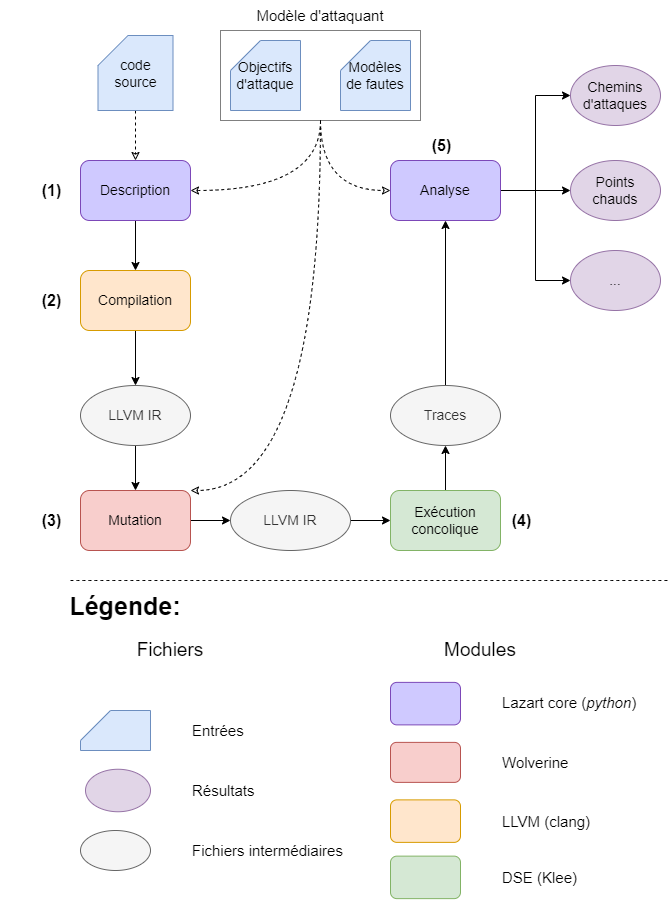
\includegraphics[scale=0.4]{ch3-lazart/img/lazart-workflow4_pack.drawio.png}
            \caption{Processus d'analyse avec Lazart}  \label{fig:lazart-analysis-scheme}
        \end{figure}
        
        Le fonctionnement indépendant des différentes étapes permet de reprendre une analyse en réutilisant les données intermédiaires des étapes précédentes, ceci afin de ne pas ré-exécuter certaines opérations coûteuses (comme l'exécution concolique). 
        Cette architecture modulaire permet aussi de simplifier l'intégration avec d'autres chaînes logicielles qui peuvent ainsi modifier une étape ou se placer entre les étapes du processus d'analyse. 
        
        Lazart est organisé en plusieurs modules: 
        \begin{itemize}
            \item \textit{Lazart Core}: une \gls{api} Python permettant la description et la manipulation des analyses, des traitements, des traces et des résultats.
            \item \textit{Wolverine}: l'outil permettant de muter un bytecode \gls{llvm} afin d'y introduire les potentielles fautes.
            \item \textit{Les outils externes} : dont notamment la chaîne de compilation de \gls{llvm} et l'outil d'exécution concolique KLEE.
        \end{itemize}
    
        Lazart Core permet à l'utilisateur de définir ses propres traitements à l'aide d'une \gls{api} en Python. Six traitements, appelés ici \og analyses \fg{}, sont proposés nativement dans Lazart:
        \begin{itemize}
            \item \textit{Recherche d'attaques}: recherche des chemins d'attaques.
            \item \textit{Analyse d'équivalence} : élimination des attaques \og équivalentes \fg{} (voir section \ref{sec:lazart-equivalence}).
            \item \textit{Analyse de redondance} : élimination des attaques \og redondantes \fg{} (voir section \ref{sec:lazart-redundancy}).
            \item \textit{Analyse de points chauds} : identification des points d'injection les plus sensibles (voir section \ref{sec:hotspots}).
            \item \textit{Analyses de placement de contre-mesures} : recherche des placements optimaux pour des contre-mesures \og locales \fg{} (décrites dans le chapitre \ref{chpt:placement}).
            \item \textit{Analyse d'optimisation de contre-mesures} : recherche des protections superflues ou redondantes dans une programme protégé  (décrite dans le chapitre \ref{chpt:ccpo}).
        \end{itemize}
            
        Lazart supporte trois modèles de faute: 
        \begin{itemize}
            \item \textit{L'inversion de test} (\gls{TI}): qui correspond à la sélection de la mauvaise branche lors d'un branchement conditionnel (instruction \texttt{br}).
            \item \textit{La mutation de données} (\gls{DL}): la donnée lue lors de l'exécution d'une instruction \texttt{load} est modifiée, la valeur injectée étant laissée au choix de l'utilisateur (valeur fixe ou valeur symbolique, éventuellement contrainte).
            \item \textit{Le saut arbitraire intra-procédural} (\gls{JMP}): la faute provoque un saut vers un point du programme (défini par l'utilisateur).
            \item[]
        \end{itemize}
        
        Ces trois modèles peuvent être combinés en multi-fautes, et permettent déjà d'exprimer un grand nombre de scénarios d'attaque.
        La suite de ce chapitre se concentre sur la description et l'utilisation des modèles de faute de Lazart pour l'utilisateur, le chapitre \ref{chpt:lazart-implem} reviendra plus en détail sur l'implémentation de ces modèles.
        
    \section{Description d'une analyse}
    \label{sec:lazart:descr}
    
        Cette section présente la description par l'utilisateur d'une analyse de recherche de chemin d'attaque avec Lazart.
        La section \ref{sec:lz:memcmps} présente la fonction \textit{memcmps} qui servira d'exemple.
        La section \ref{sec:lz:analysis-script} décrit le script d'analyse et les paramètres qui lui sont associés.
        La section \ref{sec:lazart-phi} s'intéresse à la description de l'objectif d'attaque et la section \ref{sec:lazart-am} à la description des modèles de faute.
        
        \subsection{La fonction \texttt{memcmps}}
        \label{sec:lz:memcmps}
        
            Les différentes étapes d'analyse  seront illustrées sur la fonction \texttt{memcmps} présentée dans le listing \ref{lst:example-memcmps}. 
            \texttt{memcmps} effectue une comparaison de deux tableaux d'octets en appelant plusieurs fois la fonction \texttt{memcmp} de la bibliothèque standard C de manière à se protéger contre des fautes. Si une faute sur la donnée ou une inversion de test fausse le résultat d'un appel à \texttt{memcmp}, la variable \texttt{result} ne contiendra ni \texttt{FALSE} ni \texttt{TRUE} et l'attaque sera donc détectée. 
            On considérera l'objectif d'attaque qui consiste à obtenir le retour \texttt{TRUE} malgré des entrées différentes, et la combinaison des modèles de faute d'inversion de test et de mutation de données arbitraire (non contrainte). 
        
\lstset{caption={Fonction \texttt{memcmps}},label=lst:example-memcmps}
\begin{lstlisting}    
// memcmps.h
typedef BOOL uint16_t;
#define TRUE    0x1234u
#define FALSE   0x5678u
#define MASK    0xABCDu

// memcmps.c
#include "memcmps.h"

BOOL memcmps(uint8_t* a, uint8_t* b, size_t len)
{
  BOOL result = FALSE;
  
  if (!memcmp(a, b, len)) {
    result ^= MASK;           // result = FALSE ^ MASK
    if (!memcmp(a, b, len)) {
      result ^= FALSE ^ TRUE; // result = MASK ^ TRUE
      if (!memcmp(a, b, len)) {
        result ^= MASK;       // result = TRUE
      }
    }
  }

  return result;
}
\end{lstlisting}
        
        \subsection{Script d'analyse et paramètres}
        \label{sec:lz:analysis-script}
            
            L'utilisateur décrit les paramètres et les traitements d'une analyse dans un \textit{script d'analyse} et en instrumentant le programme étudié.
            Le listing \ref{lst:vp-lazart-script} correspond au script d'analyse pour l'exemple \texttt{memcmps}.
            Ce script contient tout d'abord l'importation de Lazart (ligne 2). Les paramètres d'une analyse sont définis dans un objet de type \textit{Analysis}. Le constructeur (ligne 4) prend deux paramètres obligatoires: 
            \begin{itemize}
                \item les fichiers sources du programme: ligne 6, \texttt{memcmps.c} contenant la fonction à analyser ainsi que \texttt{main.c}, la fonction principale de l'analyse (voir section \ref{sec:lazart-phi}).
                \item le modèle d'attaquant, pour le moment représenté par la variable \texttt{attack\_model} (voir section \ref{sec:lazart-am}).
            \end{itemize}
            
\lstset{caption={Script d'analyse d'attaque pour l'exemple \texttt{memcmps}},language=python, label=lst:vp-lazart-script}
\begin{lstlisting}    
#!/usr/bin/python3
from lazart.lazart import *

a = Analysis(["memcmps.c", "main.c"], # Input files 
    attack_model, # Attack model
    flags=AnalysisFlag.AttacksAnalysis, # Analysis type
    compiler_args="-Wall",
    max_order=4,
    path="my_analysis")

execute(a)
\end{lstlisting}
            
            Un certain nombre de paramètres optionnels peuvent être spécifiés, la liste complète étant disponible dans l'annexe \ref{annexe:lz:analysis-args}.
            Dans l'exemple précédant, \texttt{flags} (ligne 6) indique les traitements qui seront effectués (ici une recherche d'attaques, \texttt{AttacksAnalysis}, la valeur par défaut).
            \texttt{compiler\_args} (ligne 7) indique les arguments supplémentaires pour l'étape de compilation et \texttt{max\_order} (ligne 8) correspond à la limite de fautes de l'analyse (par défaut 2). \texttt{path} (ligne 9) est le chemin du dossier d'analyse dans lequel les différents fichiers temporaires et les résultats seront stockés.
            
            La fonction \texttt{execute} lance les différentes étapes de l'analyse (conformément à la figure \ref{fig:lazart-analysis-scheme}) ainsi que la génération et l'affichage des résultats, en exécutant la séquence d'opérations\footnote{Dans le cadre d'une recherche de chemins d'attaques (\texttt{flag=AttacksAnalysis}) comme pour l'exemple \ref{lst:vp-lazart-script}.} indiquée dans le listing \ref{lst:vp-lazart-exec}. 
            
            \lstset{caption={Équivalent de la fonction \texttt{execute} pour une analyse d'attaque},language=python, label=lst:vp-lazart-exec}
\begin{lstlisting}    
compile_results(a) # Compilation.
run_results(a) # Mutation and DSE.
traces_results(a) # Gathering traces information from KLEE's ktests.
attacks_results(a) # Computing attacks analysis.
print_results(a) # Prints results of analysis.
generate_reports(a) # Generate analysis reports files.
\end{lstlisting}
            
            La suite de cette section explique comment l'utilisateur décrit l'objectif d'attaque et le modèle d'attaquant.

        \subsection{Description de l'objectif d'attaque}
        \label{sec:lazart-phi}
        
            L'objectif d'attaque est spécifié dans le programme à analyser.
            Le listing \ref{lst:vp-lazart-instr} présente le fichier principal de l'analyse \texttt{main.c}, instrumenté avec la spécification de l'objectif d'attaque. C'est cette fonction \texttt{main} qui sera le point d'entrée de l'exécution symbolique après l'étape de mutation.
            
            Les deux tableaux d'entrée \texttt{a1} et \texttt{a2} sont rendus symboliques à l'aide de la fonction \texttt{\_LZ\_\_SYM} (ligne 11 et 13) qui prend en paramètre le pointeur vers la zone mémoire à rendre symbolique et la taille de cette zone mémoire.
            L'objectif d'attaque est vérifié avec la macro \texttt{\_LZ\_\_ORACLE} qui limite la recherche aux d'exécutions qui valident le prédicat passé en paramètre.
            Elle permet ainsi de décrire la contrainte d'inégalité des entrées symboliques (ligne 19) et de vérifier que le retour de la fonction est \texttt{TRUE} (ligne 23).
            Les macros \texttt{\_LZ\_SYM} et \texttt{\_LZ\_ORACLE} sont implémentées à partir des directives de KLEE, respectivement \texttt{klee\_make\_symbolic} et \texttt{klee\_assume} (section \ref{sec:klee}).
             
\lstset{style=codeC, caption={Fonction principale de l'analyse},label=lst:vp-lazart-instr}
\begin{lstlisting}   
// main.c
#include "lazart.h"
#include "memcmps.h"

#define SIZE 4

int main()
{  
    // Inputs
    uint8_t a1[SIZE];
    _LZ__SYM(a1, SIZE); // Symbolic array
    uint8_t a2[SIZE];
    _LZ__SYM(a2, SIZE); // Symbolic array
    
    bool equals = true;
    for(size_t i = 0; i < SIZE; ++i)
        if(a1[i] != a2[i])
            equals = false;
    _LZ__ORACLE(!equal); // Consider only different inputs
    
    BOOL res = memcmps(a1, a2, SIZE); // Call studied function

    _LZ__ORACLE(res == TRUE); // Attack objective
}
\end{lstlisting}
        
        \subsection{Description des modèles de faute}
        \label{sec:lazart-am}
        
            Les modèles de faute peuvent être spécifiés de deux manières:
            \begin{itemize}
                \item dans le script d'analyse en Python (via l'argument \texttt{attack\_model}), permettant une granularité de l'ordre des fonctions ou des blocs de base.
                \item en instrumentant le code, ce qui permet un contrôle plus précis.
            \end{itemize}

            \begin{table}[h]
                \small
                \centering
\begin{tabular}{|l|cc|cc|}
\hline
\multicolumn{1}{|c|}{\multirow{2}{*}{Modèle}} & \multicolumn{2}{c|}{Description} & \multicolumn{2}{c|}{Granularité} \\ \cline{2-5} 
\multicolumn{1}{|c|}{} & \multicolumn{1}{c|}{Python} & Instr. & \multicolumn{1}{c|}{Python} & Instr. \\ \hline
Inversion de test (TI) & \multicolumn{1}{c|}{Oui} & Oui & \multicolumn{1}{c|}{\begin{tabular}[c]{@{}c@{}}Fonctions et blocs de\\ base\end{tabular}} & Branchements \\ \hline
\begin{tabular}[c]{@{}l@{}}Mutation de donnée (DL\\  - mutation de constantes\end{tabular} & \multicolumn{1}{c|}{\begin{tabular}[c]{@{}c@{}}Oui\\ Non\end{tabular}} & \begin{tabular}[c]{@{}c@{}}Oui\\ Oui\end{tabular} & \multicolumn{1}{c|}{\begin{tabular}[c]{@{}c@{}}Fonctions, blocs de base\\ et variables\end{tabular}} & Instructions \\ \hline
Saut arbitraire JMP) & \multicolumn{1}{c|}{Non} & Oui & \multicolumn{1}{c|}{N/ A} & Instructions \\ \hline
\end{tabular}
                \caption{Définition et granularité des modèles de faute}
                \label{tbl:lz:models-def}
                \end{table}
                
            La table \ref{tbl:lz:models-def} indique la granularité de chaque modèle de faute en fonction de la méthode de définition utilisée. La colonne \textit{Description} détermine si le modèle de faute peut être défini avec chaque méthode et la colonne \textit{Granularité} précise le niveau de granularité pour chaque méthode.
            La description en Python associe des modèles de faute à des portions de programme (fonction ou bloc de base), mais n'est disponible que pour l'inversion de test et la mutation de données.
            
            La suite de cette section explique comment ces modèles de faute sont décrits par l'utilisateur. 
        
            \subsubsection{Description du modèle d'attaquant en Python}
            \label{sec:lazart-am-py}
            
                La description du modèle d'attaquant en Python est faite en associant des modèles de faute à des fonctions ou des blocs de base du programme.
                Le listing \ref{lst:attack-model-python} présente un exemple de définition d'un modèle d'attaquant \texttt{am} composé de trois modèles de faute.
                L'annexe \ref{annexe:lz:param-analysis} décrit l'ensemble des paramètres disponibles pour chaque modèle de faute.
                
\lstset{caption={Exemple de modèle d'attaquant décrit en Python}, language=python, label=lst:attack-model-python}
\begin{lstlisting}  
model_ti = { "type": "test-inversion" }

model_breset = { 
    "type": "data-load",
    "all": 0 # All load are faulted to 0
    "exclude": ["i", "tmp"] # Except variables 'i' and 'tmp'.
}

model_gl = {
    "type": "data-load",
    "vars": {
        "my_global": "__sym__" # Arbitrary (unconstrained) value.
    }
}

am = {
    "functions": { # Associate models to functions.
        "__all__": [model_gl], # All functions
        "foo": [model_ti, model_breset]
    }
}
\end{lstlisting} 
                
                Dans l'exemple ci-dessus un modèle d'inversion de test (\texttt{model\_ti}) est appliqué sur la fonction \texttt{foo} avec le modèle de mutation de mise-à-zero (\texttt{model\_breset}). Le modèle \texttt{model\_gl} injecte une valeur arbitraire pour toute lecture de la variable \texttt{my\_global} (avec le mot clef \texttt{\_\_sym\_\_}). 
                Le champ \texttt{functions} permet l'application des modèles de faute sur des fonctions du programme (le champ \texttt{basic-blocks} est l'équivalent pour les blocs de base).
                
                Le listing \ref{lst:memcmps-am} présente le modèle d'attaquant pour l'exemple \texttt{memcmps} afin d'obtenir une combinaison de l'inversion de test et de la mutation de données. Une mutation en donnée arbitraire est appliquée sur les variables \texttt{result} et \texttt{len} et l'inversion de test est appliquée sur l'ensemble de la fonction.
                La ligne 14 est une version plus compacte de la définition de ce même modèle utilisant des fonctions utilitaires: \texttt{function\_list} associe un ensemble de modèles de faute à une liste de fonctions, et \texttt{ti\_model} et \texttt{data\_model} permettent de créer un modèle avec le champ \texttt{type} correspondant.
                
\lstset{caption={Modèle d'attaquant pour l'exemple \texttt{memcmps}}, label=lst:memcmps-am}
\begin{lstlisting}  
attack_model = {
    "functions" = {
        "memcmps" = [ {
                "type": "test-inversion"
            },
            { 
                "type": "data-load",
                "vars": { "result": "__sym__", "len":  "__sym__" }
            }
        ]
    }
}

attack_model = functions_list(["memcmps"], [ti_model(), data_model({ "vars": { "result": "__sym__", "len":  "__sym__" } })])
\end{lstlisting} 
                
            \subsubsection{Spécification du modèle de mutation de données}
            \label{sec:data-value}
        
                Le modèle de mutation de données de Lazart vise la généricité en laissant l'utilisateur spécifier la valeur qui sera injectée. Cette valeur peut être une constante, une valeur contrainte par un prédicat (encodé par une fonction définie par l'utilisateur dans le programme source) ou entièrement symbolique (non contrainte) pour le type donné. 
                Le listing \ref{lst:data-yaml-values} contient un exemple de description de la mutation de données pour chacun de ces cas.
    
\lstset{caption={Différentes spécifications de valeurs fautées en Python},label=lst:data-yaml-values}
\begin{lstlisting}  
{
    "type": "data-load",
    "vars": {
        "x": 0,               # Fixed value
        "y": "my_predicate",  # Constrained symbolic
        "z": "__sym__",       # Not-constrained symbolic
    }
}
\end{lstlisting}                 
                    
                Le listing \ref{lst:data-predicate-function} présente un exemple de deux prédicats \texttt{flip\_pred} et \texttt{bf\_pred} encodant respectivement le modèle d'inversion de tous les bits (\textit{flip}) et le modèle d'inversion d'un seul bit (\textit{bit-flip}), implémenté en langage C. Un prédicat prend en entrée la valeur originale (potentiellement symbolique) et la valeur injectée (toujours symbolique). 
               
\begin{lstlisting}[caption={Prédicat pour le modèle \textit{bit-flip}}, label=lst:data-predicate-function, language=C,style=codeC]
bool bf_pred(int value, int faulted)
{
    return hamming_distance(value, faulted) == 1; // on binary encoding.
}

bool flip_pred(int value, int faulted)
{
    return faulted == ~value;
}
\end{lstlisting}        
                    
                La table \ref{tbl:data-modele-mode} présente les types de mutation de données de Lazart permettant de représenter certains modèles de faute de la littérature.
                La première colonne indique le modèle de faute considéré et les colonnes suivantes indiquent si la méthode correspondante peut être utilisée (\textit{oui}) ou \textit{non}, \textit{possible} indiquant que la méthode peut représenter le modèle mais n'est pas la plus adaptée. 
                
                L'approche par \textit{prédicat} est la plus générique, pouvant s'appliquer dans tous les cas, la \textit{valeur fixe} et la valeur non-contrainte (\textit{symbolique}) étant réservées à des cas spécifiques.
                Le chapitre suivant (section \ref{sec:lazart-mfct-data}) s'intéresse aux considérations liées aux performances de l'analyse dans le choix de la fonction de mutation associé à chaque type de valeur fautée.
                
                \begin{table}[ht]
                \centering
                \small
                    \begin{tabular}{|l|c|c|c|}
                    \hline
                    Modèles de la littérature                                                     & \multicolumn{1}{l|}{Valeur fixe} & \multicolumn{1}{l|}{Symbolique} & \multicolumn{1}{l|}{Prédicat} \\ \hline
                    \begin{tabular}[c]{@{}l@{}}bit-set\\ bit-reset\end{tabular}   & possible                       & non                             & oui                           \\ \hline
                    bit-flip                                                      & non                              & non                             & oui                           \\ \hline
                    \begin{tabular}[c]{@{}l@{}}byte-set\\ byte-reset\end{tabular} & oui                              & non                             & oui                           \\ \hline
                    byte-flip                                                     & non                              & non                             & oui                           \\ \hline
                    \begin{tabular}[c]{@{}l@{}}set\\ reset\end{tabular}           & oui                              & non                             & possible                      \\ \hline
                    inversion                                                     & non                              & non                             & oui                           \\ \hline
                    valeur aléatoire                                              & non                              & oui                             & possible                      \\ \hline
                    valeur arbitraire                                             & non                              & oui                             & oui                           \\ \hline
                    \end{tabular}
                                \caption{Modèle de faute sur les données \label{tbl:data-modele-mode}}
                \end{table}
                    
            \subsubsection{Mutation par instrumentation}
            \label{sec:lazart-am-instr}
                
                L'instrumentation du programme est complémentaire à la description du modèle d'attaquant en Python. L'instrumentation peut être utilisée afin :
                \begin{itemize}
                    \item d'obtenir un contrôle plus fin sur l'application des modèles de faute.
                    \item de définir un point d'injection spécifique dans le programme.
                    \item de spécifier un modèle de faute non disponible via l'\gls{api} Python (saut arbitraire).
                \end{itemize}

                \begin{sloppypar}
                Le listing \ref{lst:instr-enable} présente une fonction \texttt{foo} contenant des macros de Lazart permettant le contrôle de l'activation de modèles. Les fonctions \texttt{\_LZ\_\_disable\_model}, et \texttt{\_LZ\_\_enable\_models} permettent respectivement de désactiver un modèle nommé (à l'aide du champ \texttt{name} d'un modèle de faute) et de réactiver tous les modèles.
                Ces fonctions doivent être placées en prenant en compte l'ordre dans lequel le compilateur va placer les blocs de base dans la représentation \gls{llvm-ir}\footnote{Cela dépend du compilateur et de sa version mais l'utilisateur peut inspecter le code \gls{llvm-ir} généré en cas d'ambiguïté.}.
                L'état d'activation des modèles n'est pas préservé entre les fonctions. 
                La fonction \texttt{\_LZ\_\_disable\_bb} permet ici de désactiver tous les modèles dans un bloc de base.
                \end{sloppypar}
                       
\lstset{style=codeC, caption={Activation et désactivation de modèles},label=lst:instr-enable}
\begin{lstlisting}     
int foo(int i, float f)
{
    _LZ__disable_model("fm:ti"); // Disable a named fault model.
    int ret = 0;
    if(a < 0)
    {
        _LZ__disable_bb(); // Disable all models in the current basic block.
        ret = a * f;
    }
    else
    {
        ret = bar(a * f);
    }
    _LZ__enable_models(); // Enable all disabled models.
    
    return ret;
}
\end{lstlisting}

                Le listing \ref{lst:instr-inplace} présente une fonction \texttt{bar} contenant des points d'injection définis manuellement. La fonction \texttt{\_LZ\_\_DATA\_i32} (ligne 6) permet de spécifier un point d'injection de mutation de données sur la constante \texttt{10} correspondant à la limite de boucle, le second paramètre est l'identifiant du point d'injection.
                Aux lignes 4 et 5, deux points d'injection de sauts d'instruction (\texttt{lend} et \texttt{end}) sont définis avec la macro \texttt{\_LZ\_\_JUMP}. La faute provoque un saut respectivement aux labels \texttt{loop\_end} (ligne 9) et \texttt{end} (ligne 12).
                        
\lstset{style=codeC, caption={Définition manuelle de points d'injection},label=lst:instr-inplace}
\begin{lstlisting}     
int bar(int a, int b)
{
    int total = 0;
    _LZ__JUMP(loop_end, "lend"); // (label, id)
    _LZ__JUMP(end, "end"); // (label, id)
    for(int i = 0; a < _LZ__DATA_i32(10, "loop_bound"); ++i) // (original, id)
    {
        total += a + b;
        loop_end:
    }
    
    end:
    return foo(total);
}
\end{lstlisting}               

    \section{Traces et traitements}
    \label{sec:lazart-formal}
     
        Les différents traitements de Lazart prennent en entrée un ensemble de traces d'exécution qui sont obtenues à partir des cas de tests de KLEE.
        Cette section présente la modélisation des traces au sein de Lazart (section \ref{sec:lz:traces}) et décrit les différentes analyses de robustesse de Lazart: \textit{l'analyse d'attaque} (section \ref{sec:lazart-aa}), \textit{l'analyse d'équivalence} (section \ref{sec:lazart-equivalence}), \textit{l'analyse de redondance} (section \ref{sec:lazart-redundancy}) et \textit{l'analyse de points chauds} (section \ref{sec:hotspots}).

        \subsection{Représentation des traces dans Lazart}
         \label{sec:lz:traces}

            Comme cela a été vu dans la section \ref{sec:dse-fi}, l'exécution concolique sur le mutant embarquant les fautes revient à une exploration de tous les chemins fautés\footnote{Dans le cas idéal, c'est-à-dire dans le cas où l'exécution concolique est complète. Les chemins fautés dépassant la limite de fautes fixée par l'utilisateur ne sont pas explorés.}. 
            Chaque cas de test généré par KLEE peut être vu comme une trace d'exécution représentant un ensemble d'exécutions qui suivent le même chemin et comprennent les mêmes déclenchements de fautes.
            Les valeurs concrètes (pour les entrées et les fautes) d'un cas de test permettent d'obtenir un représentant de cet ensemble d'exécutions.
            
            \begin{figure}[t]\centering
              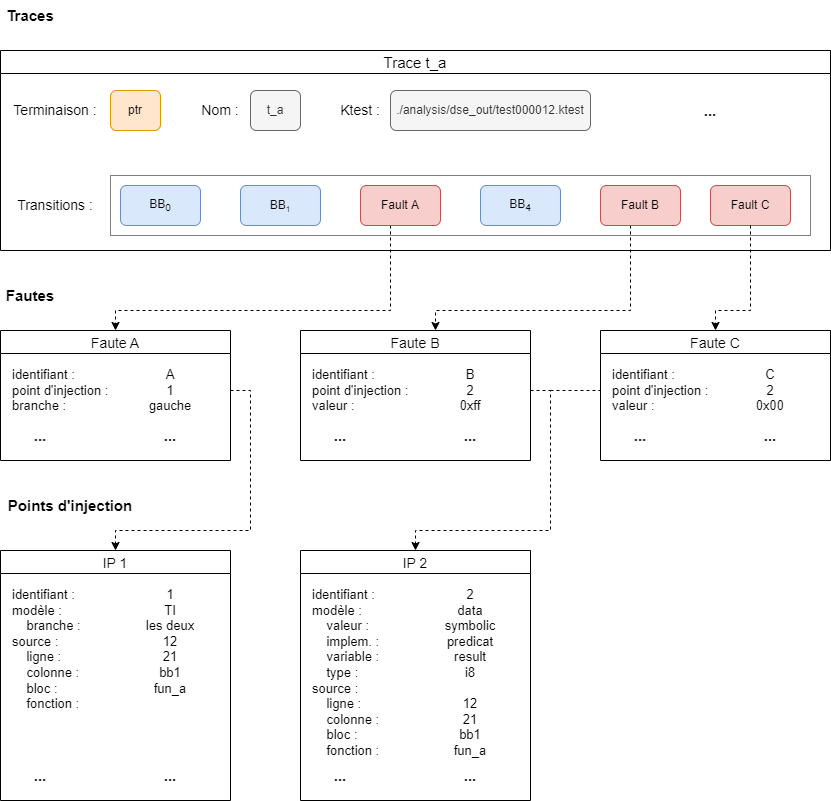
\includegraphics[scale=.43]{ch3-lazart/img/trace-model.drawio.png}
              \caption{Représentation d'une trace d'attaque dans Lazart \label{fig:lz-trace-model}}
            \end{figure}
            
            Ces traces d'exécution sont représentées dans Lazart par un type de \textit{terminaison}, et une liste ordonnée de \textit{transitions} pouvant être du type: 
            \begin{itemize}
                \item \textit{bloc de base}: entrée dans un bloc de base.
                \item \textit{faute}: un point d'injection a été déclenché.
            \end{itemize}
            
            \begin{defi}
                Soit $P$ un programme et $m$ un modèle de faute, on note $T(P, m)$ l'ensemble des traces d'exécution de $P$, ou plus simplement $T(P)$.
            \end{defi}
            
            Les transitions correspondant à l'entrée dans un bloc de base permettent de tracer le flot d'exécution. 
            Les transitions fautées sont paramétrées par le point d'injection déclenché (et donc le modèle de faute correspondant) et les paramètres de la faute. 
            Le type de terminaison d'une trace $t$, notée $Term(t)$, correspond aux terminaisons des cas de tests de KLEE\footnote{Pour rappel: \texttt{ptr}, \texttt{div}, \texttt{free}, \texttt{abord}, \texttt{assert}, \texttt{model}, \texttt{satisfy}, \texttt{timeout} etc.} (section \ref{sec:klee}) étendues avec la terminaison en contre-mesure (\texttt{detected}) et des cas d'erreurs supplémentaires spécifiques à Lazart (\texttt{lzerrs}).
            
            \begin{defi}
                Soit $t \in T(P)$, on note: 
                \begin{itemize}
                    \item $Tr(t)$ la liste ordonnée des transitions dans $t$.
                    \item $N(t)$ la liste ordonnée des transitions non fautées dans $t$.
                    \item $F(t)$ la liste ordonnée des transitions fautées dans $t$.
                \end{itemize}
            \end{defi}
        
            La figure \ref{fig:lz-trace-model} donne la représentation d'une trace d'exécution \texttt{t\_a} contenant la faute $A$ en inversion de test et les fautes $B$ et $C$ en mutation de données et deux points d'injection.
            
        \subsection{Analyse d'attaque}
        \label{sec:lazart-aa}
            
            L'analyse d'attaque correspond à la recherche de chemins d'attaques validant un objectif d'attaque $\phi$.
            
            \begin{defi}
                Une \textit{attaque} est une trace d'exécution comportant au moins une faute: $F(t) \neq \emptyset, t \; \in T(P)$.
            \end{defi}
            
            \begin{defi}
                Une \textit{attaque réussie}, pour un objectif d'attaque $\phi$, est une attaque validant l'objectif d'attaque: $F(t) \neq \emptyset \; \land t \vDash \phi, \; t \in T(P)$.
                
            \end{defi}
            
            La table \ref{tbl:memcmps-aa-results} donne le nombre de chemins d'attaque trouvés pour notre exemple avec une limite de fautes fixée à 4, et avec le modèle de faute combiné d'inversion de test et de mutation de données sur \texttt{result} et \texttt{i}. La taille des tableaux d'entrées est fixée à 4 et leurs valeurs sont symboliques (et contraintes d'être différentes sur au moins un octet
        
            \begin{table}[h]
                \caption{Chemins d'attaque trouvés avec \texttt{memcmps}}
                \label{tbl:memcmps-aa-results}
                \small
                \begin{center}
                    \begin{tabular}{l|llllll}
                    Fautes & 1F & 2F & 3F & 4F & 5F & Total \\
                    \hline
                    Attaques réussies & 0 & 4 & 8 & 20 & 28 & 60
                    \end{tabular}
                \end{center}
            \end{table}  
        
            \begin{figure}[!htp]\centering
                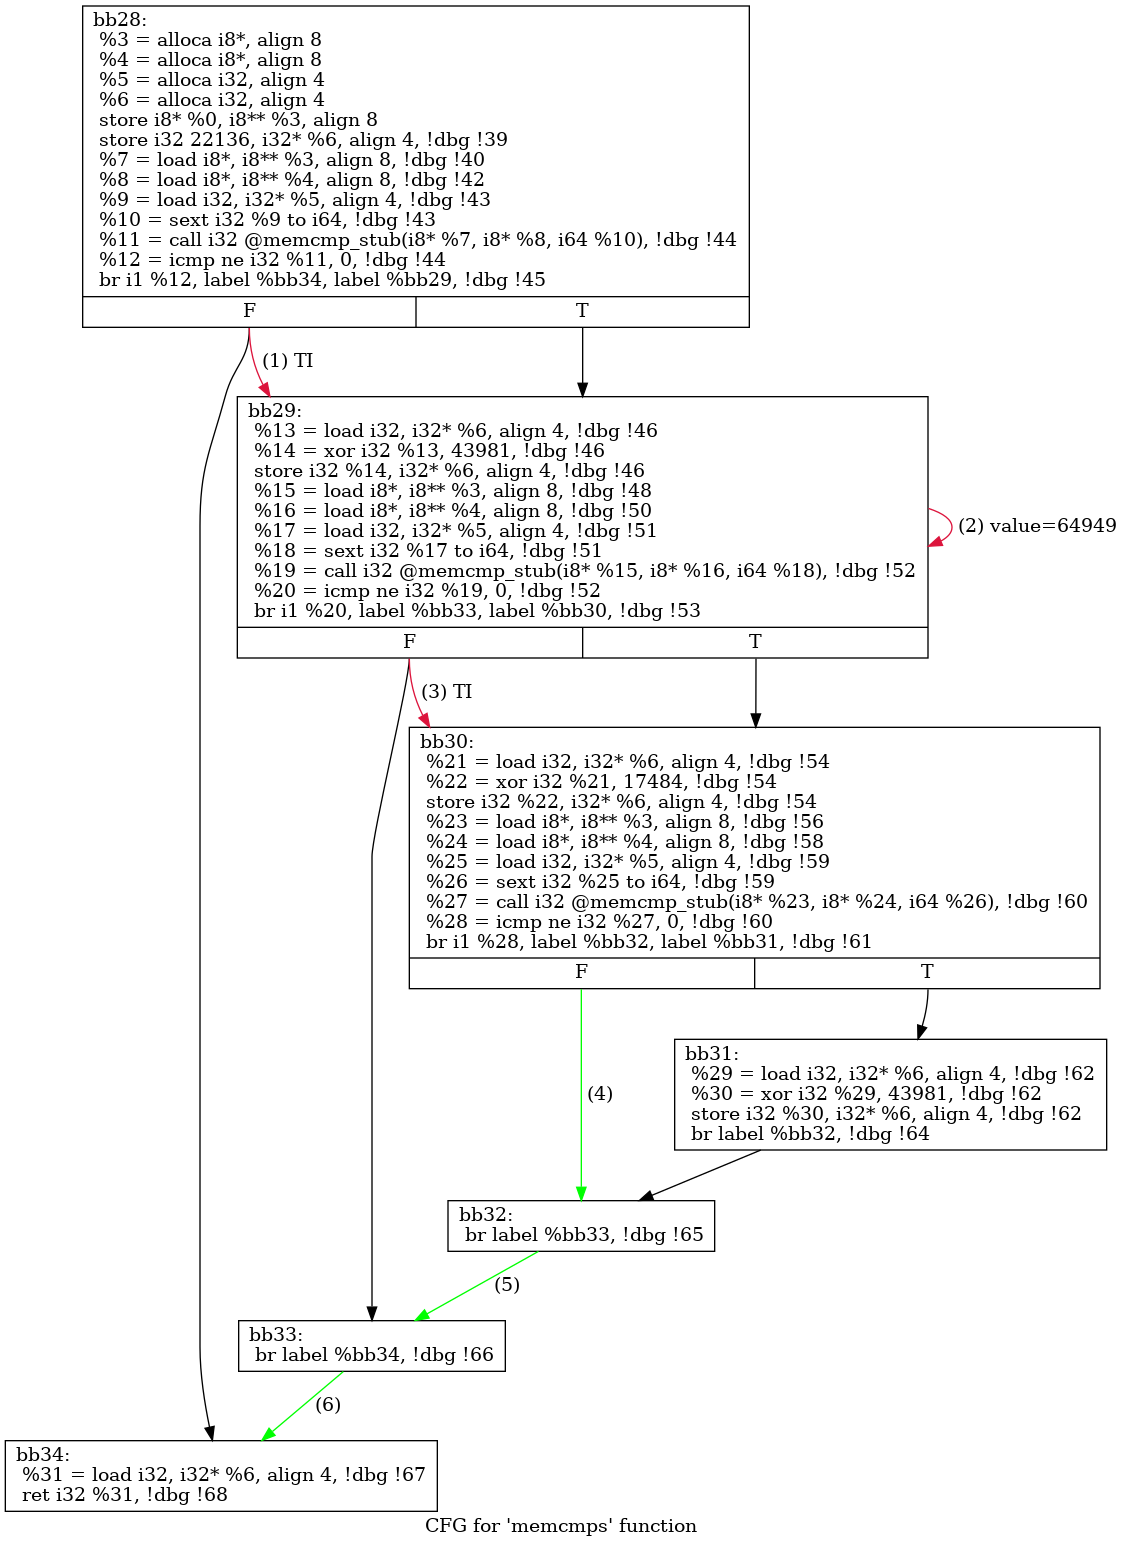
\includegraphics[scale=0.35]{ch3-lazart/img/cfg.memcmps.png}
                \caption{Graphe de faute de l'attaque en trois fautes sur \texttt{memcmps}}  \label{fig:memcmps-lazart-trace-graph}
            \end{figure}
        
            Le listing \ref{lst:memcmps-trace} présente une trace en trois fautes composée de deux inversions de test et une mutation de donnée.
            On y trouve en premier lieu le nombre de fautes dans la trace (\texttt{3}), son nom (\texttt{t15}) puis la liste ordonnée des transitions\footnote{Ici chaque faute indique dans l'ordre : l'identifiant du point d'injection concerné, le modèle de faute (ici \texttt{TI} ou \texttt{DL}), les informations spécifiques au modèle et finalement les informations sur la position du point d'injection dans le code source.}. Finalement le mot-clef \texttt{Satisfy} correspond au type de terminaison (ici l'objectif d'attaque a été validé).
            
            La figure \ref{fig:memcmps-lazart-trace-graph} correspond au graphe d'attaque généré par Lazart pour cette attaque. Le chemin suivi dans le graphe de flot de contrôle du programme étudié est indiqué en vert et les fautes sont indiquées en rouge.
            Cette attaque consiste à inverser le test du premier appel à \texttt{memcmp} (ligne 14\footnote{Voir code de \texttt{memcmps} dans le listing \ref{lst:example-memcmps}.}), puis injecter la valeur $FALSE \oplus MASK$ ($0x5678 \oplus 0xABCD = 64949$) dans la variable \textit{result} (ligne 15) et enfin inverser le test ligne 16. La ligne 17 est ainsi exécutée, on a $result = result \oplus FALSE \oplus TRUE \implies result = FALSE \oplus FALSE \oplus TRUE = TRUE$. Le dernier test n'est pas fauté et la ligne 19 n'est pas exécutée, la valeur $TRUE$ est donc retournée par la fonction.
                
    \lstset{caption={Attaque en trois fautes sur \texttt{memcmps}},language=python, label=lst:memcmps-trace}
\begin{lstlisting}   
(<3> t15: [BB(bb28), FAULT(0|TI|: bb28 => bb29 [l:27, bb:bb28]), BB(bb29), FAULT(1|DL|: ~ => 64949 [l:28, bb:bb29]), FAULT(2|TI|: bb29 => bb30 [l:29, bb:bb29]), BB(bb30), BB(bb32), BB(bb33), BB(bb34)]: Satisfy)
\end{lstlisting}               
                    
            \begin{sloppypar}
            Comme toutes les analyses de Lazart, l'analyse d'attaque prend l'argument \texttt{satisfies\_fct} correspondant à un prédicat déterminant si une trace valide l'objectif d'attaque ou non afin de laisser un contrôle fin à l'utilisateur. 
            Cela permet d'exprimer des objectifs d'attaque qui ne peuvent pas être décrits uniquement par l'instrumentation (par exemple des erreurs à l'exécution). 
            Le listing \ref{lst:s_fct} présente la définition d'un prédicat considérant comme une attaque les traces finissant en erreur arithmétique ou d'adresse, en plus des exécutions validant l'objectif d'attaque\footnote{Par défaut, seules les traces avec pour type de terminaison \textit{satisfy} sont prises en compte.}.
            La liste complète des paramètres des différentes analyses est donnée dans l'annexe \ref{annexe:lz:param-analysis}.                    
            \end{sloppypar}
                
    \lstset{caption={Filtrage des traces d'attaque en fonction de la terminaison},language=python, label=lst:s_fct}
\begin{lstlisting}    
Term = TerminationType # alias
attacks_analysis(satisfies_fct=lambda trace: trace.termination_is(Term.Satisfy, Term.Ptr, Term.Div, Term.Free))
\end{lstlisting}   
            
        \subsection{Équivalence des attaques et entrées symboliques}
        \label{sec:lazart-equivalence}
            
            Lazart propose les notions d'\textit{équivalence} et de \textit{redondance} (abordée en section \ref{sec:lazart-redundancy}) qui forment une relation d'ordre partiel entre les attaques permettant de présenter en priorité certaines attaques à l'utilisateur.
            Ces notions visent à aider à la protection et l'évaluation du code, en permettant de cibler les attaques jugées plus importantes.   
            
            Deux définitions d'équivalence sont proposées par Lazart nativement. Elles visent chacune à regrouper entre-elles des traces d'attaques selon des objectifs différents:
            \begin{itemize}
                \item[] \textbf{1)} \textit{Équivalence} (section \ref{sec:eq}): vise à pallier à une problématique relative à une division de certains chemins d'attaques, en raison du code implémentant la vérification de l'objectif d'attaque dans le cadre d'entrées symboliques.
                \item[] \textbf{2)} \textit{Faute-équivalence} (section \ref{sec:feq}): vise à regrouper des attaques qui ne diffèrent que par des variations légères et que l'on souhaite ne pas distinguer pour l'utilisateur.
            \end{itemize}
        
            \subsubsection{Distinguabilité et équivalence}
            \label{sec:eq}

                \begin{defi}[Équivalence]
                    \label{def:eq}
                    Une \textit{attaque} $a$ est dite \textbf{équivalente} (noté $\equiv$) à une attaque $a'$ si leur séquence de transitions sont égales (égalité syntaxique des séquences): \\
                    $a \; \equiv \; a' \;\;=_{def} \; Tr(a) = Tr(a')$ %\wedge Term(a) = Term(a')
                \end{defi}
            
                La notion d'équivalence des attaques (définition \ref{def:eq}) vise à regrouper les attaques qui suivent le même chemin, contiennent les mêmes fautes, mais ont des contraintes sur les entrées différentes.
                On définira la \textit{distinguabilité} d'un prédicat de chemin fauté au sein d'un ensemble $\omega^M$ (définition \ref{def:pcf-distinct}) et la \textit{distinguabilité} de l'énumération des prédicats de chemins fautés (définition \ref{def:fi-distinct}).  
            
                \begin{defi}
                \label{def:pcf-distinct}
                    Un prédicat de chemin fauté $PC^M_{\omega}$ est dit \textit{distinct} dans $\mathcal{E}^M$, si pour tout modèle $m$ satisfaisant $PC^M_{\omega}$, il \textit{n'existe pas} $PC' \in \mathcal{E}^M$ tel que $m \vDash PC'$.
                \end{defi}
                
                
                \begin{defi}
                \label{def:fi-distinct}
                    L'énumération des prédicats de chemins fautés (d'une exécution symbolique fautée $\epsilon$) est \textit{distincte} si tous les prédicats de chemins sont distincts.
                \end{defi}
                
                Il est possible que l'exécution concolique fautée ne soit pas \textit{distincte}, par exemple à cause du code encodant la vérification de l'objectif d'attaque qui divise certains chemins en plusieurs chemins non distincts (équivalents).
                Le programme présenté dans le listing \ref{lst:equiv} compte le nombre d'octets nuls dans un tableau de taille donnée. 
                Une exécution symbolique sur la fonction \texttt{null\_bytes} produit quatre chemins pour \texttt{size} fixé à 2:
                \begin{itemize}
                    \item Le chemin avec: $tab[0] = 0 \land tab[1] = 0 $.
                    \item Le chemin avec: $tab[0] \neq 0 \land tab[1] = 0 $.
                    \item Le chemin avec: $tab[0] = 0 \land tab[1] \neq 0 $.
                    \item Le chemin avec: $tab[0] \neq 0 \land tab[1] \neq 0 $.
                \end{itemize}
                
                Ces quatre chemins sont distincts (les séquences de transitions ne sont pas strictement équivalentes), chacun exécutant ou non l'incrémentation (ligne 5) à chacun des deux tours de boucle. 
                
\begin{center}
\lstset{language=C,style=codeC} 
\begin{lstlisting}[caption=Fonction \texttt{null\_bytes}, label=lst:equiv]
int null_bytes(uint8_t* tab, size_t size) {
    int total = 0;
    for(int i = 0; i < size; i++)
        if(tab[i] == 0)
            total++;
    return total;
}
\end{lstlisting}
\end{center}
                    
                Un objectif d'attaque consiste à retourner la mauvaise valeur en injectant des fautes \footnote{Silent Data Corruption (\gls{sdc}).}.
                Il est nécessaire d'encoder cette propriété dans le programme et pour cela, une méthode classique consiste à appeler la fonction étudiée sans injecter de faute et comparer les résultats, comme présenté dans le listing \ref{lst:equiv-oracle}. 
                Le tableau \texttt{tab} est rendu symbolique (ligne 3) et la valeur retournée (\texttt{ret}) est comparée à une version non fautée de la fonction à étudier (ici \texttt{null\_bytes\_safe} ligne 8).
                    
\begin{center}
\lstset{language=C,style=codeC} 
\begin{lstlisting}[caption=Point d'entrée de l'analyse pour \texttt{null\_bytes}, label=lst:equiv-oracle]
int main() {
    uint8_t tab[SIZE];
    _LZ__SYM(&tab, SIZE);
    
    int ret = null_bytes(tab, SIZE);
    
    // Verify attack objectives
    _LZ__ORACLE(ret != null_bytes_safe(tab, SIZE)); // Attacks division
}
\end{lstlisting}
\end{center}                    
                Pour chaque chemin atteignant le point de vérification de l'objectif d'attaque (ligne 8), la fonction \texttt{null\_bytes\_safe} est exécutée par le moteur d'exécution concolique.
                Dans le cas d'une exécution nominale, l'appel à \texttt{null\_bytes\_safe} produit exactement les mêmes contraintes pour chaque chemin que l'appel à \texttt{null\_bytes}, seuls quatre chemins sont donc générés, aucun ne validant l'objectif d'attaque.
                Dans le cadre d'une exécution fautée, l'appel à \texttt{null\_bytes\_safe} peut diviser certains chemins d'attaque, en ajoutant des contraintes différentes de celles de \texttt{null\_bytes} en raison des fautes.
                Si un chemin est divisé en plusieurs chemin qui valident l'objectif d'attaque, plusieurs ktests sont produits par KLEE alors qu'ils suivent le même chemin (dans la fonction étudiée \texttt{null\_bytes}, mais dont le chemin diffère dans \texttt{null\_bytes\_safe}) et contiennent les mêmes points d'injection de fautes.
    
                La table \ref{tbl:eq-results-prepost} compare les résultats obtenus pour les trois variantes de l'encodage de l'objectif d'attaque:
                \begin{itemize}
                    \item \textit{fix}: le tableau d'entrée est fixé à [1, 1].
                    \item \textit{sym-post}: le tableau d'entrée est symbolique et l'objectif d'attaque est vérifié à la fin.
                    \item \textit{sym-pre}: le tableau d'entrée est symbolique et l'objectif d'attaque est vérifié à la fin, mais la valeur attendue est pré-calculée avant l'appel de la fonction à analyser.
                \end{itemize}

                \begin{table}[h]
                    \caption{Résultats d'analyse d'équivalence sur les attaques réussies pour \texttt{null\_bytes}}
                    \label{tbl:eq-results-prepost}
                    \small
                    \begin{center}
                        \begin{tabular}{l|llllll}
                                 & Chemins Expl. & Traces & Attaques    & 1 faute & 2 fautes & Total \\
                                 \hline
                        \textit{fix}      & 14 & 11  & attaques    & 7       & 4        & 11    \\
                                 &    &     & classes eq. & 7       & 4        & 11    \\
                        \textit{sym-pre}  & 14 & 11  & attaques    & 7       & 4        & 11    \\
                                 &    &     & classes eq. & 7       & 4        & 11    \\
                        \textit{sym-post} & 19 & 16  & attaques    & 9       & 7        & 16    \\
                                 &    &     & classes eq. & 8       & 4        & 12  
                        \end{tabular}
                    \end{center}
                \end{table} 
            
                La colonne "Chemins Expl." indique le nombre de chemins explorés par KLEE, et "Traces" le nombre de traces générées par Lazart.
                Les colonnes suivantes indiquent le nombre d'attaques réussies trouvées (ligne "attaques") et le nombre de classes d'équivalence obtenues (ligne "classes eq.").
                On peut constater que l'analyse est \textit{distincte} en cas de pre-vérification dans cet exemple contrairement à la post vérification. 
                Les attaques obtenues après équivalence (lignes "classes eq.") sont bien égales entre les versions \textit{sym-pre} et \textit{sym-post}, à l'exception d'une classe d'équivalence supplémentaire qui n'est pas trouvée dans le cas \textit{sym-pre}. 
                Le pré-calcul est plus efficace puisque les contraintes sur les entrées sont exprimées avant l'appel de la fonction à étudier. Par conséquent, certains chemins peuvent être coupés directement pendant l'exécution symbolique fautée de \texttt{null\_bytes}.
                La version \textit{sym-pre} est aussi plus efficace, moins de chemins étant explorés.
                La version \textit{fix} est distincte mais est incomplète par rapport à l'utilisation d'entrées symboliques.
                L'utilisateur devrait dans le cas idéal préférer calculer au plus tôt les variables nécessaires pour vérifier l'objectif d'attaque (valeur attendues, contraintes des entrées...), même si cet exemple illustre le cas où un chemin supplémentaire est obtenu dans le cas de pre-vérification.
                
                En résumé, la notion d'équivalence (définition \ref{def:eq}) permet de regrouper les attaques qui ne varient que par leurs contraintes sur les entrées\footnote{Et potentiellement qui varient aussi au niveau du chemin dans l'encodage de l'objectif d'attaque.} de manière à ne présenter que les groupes d'équivalence à l'utilisateur.

            \subsubsection{Faute-équivalence}
            \label{sec:feq}
            
                La définition d'\textit{équivalence} impose la stricte égalité des transitions des attaques.
                La définition \textit{faute-équivalence} (définition \ref{def:feq}) se concentre sur l'égalité de la liste des transitions fautées uniquement.
                Cette définition ignore ainsi les variations de chemins (transitions non fautées) entre le déclenchement des fautes. 
                
                \begin{defi}[Faute-équivalence]
                    \label{def:feq}
                    Une \textit{attaque} $a$ est dite \textbf{faute-équivalente} (noté $\sim_f$) à une attaque $a'$ si leur séquence de transitions fautées sont égales (égalité syntaxique des séquences des fautes \footnote{Seuls les points d'injection sont comparés, pas les paramètres de fautes tels que la valeur d'une donnée injectée.}): \\
                    $a \; \sim_f \; a' \;\;=_{def} \; F(a) = F(a')$ 
                \end{defi}
            
                Cette définition vise à regrouper entre-elles des attaques qui ne diffèrent que par des variations de chemins liées aux entrées mais contiennent les mêmes fautes. Parmi ces différences qui sont captées par la \textit{faute-équivalence}:
                \begin{itemize}
                    \item des attaques qui diffèrent par un branchement n'ayant pas d'impact sur l'objectif d'attaque.
                    \item des attaques qui diffèrent par des fautes injectées à des itérations différentes dans une boucle.
                \end{itemize}
                
                La table \ref{tbl:aeq-results} compare les résultats obtenus pour \texttt{null\_bytes} avec les deux définitions de l'équivalence et donne les résultats obtenus pour l'inversion de test avec un objectif d'attaque visant à retourner un résultat incorrect (\gls{sdc}).
                La ligne \textit{attaques} correspond au total d'attaques réussies avant l'analyse d'\textit{équivalence}.
                La suivante correspond aux résultats d'équivalence et la troisième aux résultats de \textit{faute-équivalence}.

                \begin{table}[ht]
                    \caption{Comparaison des définitions de l'équivalence sur \texttt{null\_bytes}}
                    \label{tbl:aeq-results}
                    \small
                    \begin{center}
                        \begin{tabular}{l|llllll}
                        Fautes & 1F & 2F & 3F & Total \\
                        \hline
                        attaques & 13 & 5 & 0 & 18\\
                        classes d'équivalence & 11 & 4 & 0 &  15 \\
                          %- dont singletons & 10 & 3 & 0 & 13 \\
                        classes de faute-équivalence & 2 & 2 & 0 & 4\\
                          %- dont singletons & 0 & 0 & 0 & 0 \\
                        \end{tabular}
                    \end{center}
                \end{table} 
            
                Seules deux classes de faute-équivalence en une faute sont trouvées:
                \begin{itemize}
                    \item L'attaque consistant à inverser la condition d'entrée dans la boucle \texttt{for} (ligne 3). Cette attaque ne fonctionne que si le tableau d'entrée n'est pas "[0, 0]".
                    \item l'attaque consistant à inverser une des deux itérations afin de fausser le résultat.
                \end{itemize}
            
                \begin{table}[ht]
                    \caption{Comparaison des définitions de l'équivalence sur \texttt{memcmps}}
                    \label{tbl:aeq-memcmps-results}
                    \small
                    \begin{center}
                        \begin{tabular}{l|llllll}
                        Fautes & 1F & 2F & 3F & 4F & 5F & Total \\
                        \hline 
                        attaques & 4 & 8 & 20 & 28 & 28 & 88\\
                        classes d'équivalence & 1 & 2 & 5  & 7 & 7 & 22\\
                          %- dont singletons & 0 & 0 & 0 & 0  & 0 & 0\\
                        classes de faute-équivalence & 1 & 2 & 5  & 7 & 7 & 22\\
                          %- dont singletons & 0 & 0 & 0 & 0  & 0 & 0\\
                        \end{tabular}
                    \end{center}
                \end{table} 

            
            La table \ref{tbl:aeq-memcmps-results} présente de la même manière les résultats obtenus avec la fonction \texttt{memcmps}.
            On peut constater que, dans cet exemple, les définitions d'équivalence et de faute-équivalence fournissent les mêmes classes, seul le regroupement des chemins non distincts a un impact\footnote{\texttt{memcmps} \textit{n'ayant pas de boucle (fautée), les attaques ne diffèrent pas par les itérations de boucle.}}. 
        
        \subsection{Redondance des attaques} 
        \label{sec:lazart-redundancy}
        
            La notion de \textit{redondance} des attaques vise également à sélectionner les attaques qui seront à regarder en priorité par l'utilisateur.
            On considère qu'une attaque $a'$ est \textit{redondante} par rapport à une attaque $a$, si $a'$ est une variation de $a$ avec des fautes supplémentaires, noté $a < a'$.
            L'idée sous-jacente est que protéger les \textit{attaques minimales} (définition \ref{def:redun-minimal}), protégera probablement les attaques redondantes qui leurs sont liées.
            
            \begin{defi}[Terminologie]
                \label{def:redun-minimal}
                Soit $<$ un ordre partiel correspondant à une relation de redondance, une attaque $a \in T_s(P)$ est dite \textit{minimale} si elle n'est redondante par rapport à aucune autre attaque:
                    \[  
                    Min(a) =_{def} \nexists \; a' \in T_s(P) \mid a > a' \land a \neq a'
                    \] 
                On note $Red(a)$ l'ensemble des attaques redondantes par rapport à $a$.
            \end{defi}
            
            \subsubsection{Préfixe et sous-mot}
            
            Lazart propose deux définitions pour la redondance des attaques: \textit{préfixe} (définition \ref{def:redun-prefix}) et \textit{sous-mot} (définition \ref{def:redun-subword}).
            
            \begin{defi}[Redondance par préfixe]
                \label{def:redun-prefix}
                Une \textit{attaque} $a'$ est \textit{redondante par préfixe}, noté $<_p$, par rapport à une attaque $a$, si le mot des transitions fautées de $a$ $(F(a))$ est un \textbf{préfixe propre} du mot $F(a')$.
            \end{defi}
            
            \begin{defi}[Redondance par sous-mot]
                \label{def:redun-subword}
                Une \textit{attaque} $a'$ est \textit{redondante par sous-mot}, noté $<_s$, par rapport à une attaque $a$, si $F(a)$ est un \textbf{sous-mot strict} du mot $F(a')$.
            \end{defi}
            
            La définition \textit{préfixe} se concentre sur les attaques où les fautes supplémentaires sont situées après un préfixe commun, ce qui apporte une garantie que les fautes redondantes de $a'$ n'ont pas d'impact sur le préfixe.
            La définition\textit{ sous-mot} autorise que des fautes redondantes soient injectées entre les fautes communes.
        
            La table \ref{tbl:memcmps-aar-results} présente les résultats de l'analyse de redondance et d'équivalence sur l'exemple \texttt{memcmps}. 
            Chaque colonne indique le nombre d'attaques obtenues pour un nombre de fautes donné, la dernière colonne indiquant le total.
            La première ligne correspond au nombre d'attaques réussies pour chaque nombre de fautes et la seconde aux attaques réussies minimales.
            Les deux dernières lignes correspondent respectivement aux classes d'équivalence et aux classes d'équivalence minimales, avec la définition de faute-équivalence. Les classes d'équivalence minimales sont des classes d'équivalence d'attaques minimales\footnote{Les attaques d'une classe d'équivalence sont toutes minimales ou toutes redondantes.}.
            Se concentrer sur les classes d'équivalence minimales, permet donc de réduire le nombre d'attaques à considérer pour l'utilisateur.
            
            \begin{table}[h]
                \caption{Attaques minimales trouvées pour \texttt{memcmps}}
                \label{tbl:memcmps-aar-results}
                \small
                \begin{center}
                    \begin{tabular}{l|llllll}
                    Fautes & 1F & 2F & 3F & 4F & 5F & Total \\ 
                    \hline
                    Attaques réussies & 0 & 4 & 8 & 20 & 28 & 88 \\ 
                    Attaques réussies minimales & 0 & 4 & 4 & 8 & 0 & 16 \\ 
                    Classes fautes-équivalence & 0 & 1 & 2 & 5 & 7 & 22 \\ 
                    Classes fautes-équivalence minimales & 0 & 1 & 1 & 2 & 0 & 4
                    \end{tabular}
                \end{center}
            \end{table}  
            
            \subsubsection{Combinaison des notions d'équivalence et de redondance}
            
                La recherche des attaques minimales nécessite simplement de déterminer si chaque attaque est redondante par rapport à au moins une attaque, mais pas nécessairement de trouver $Red(a)$ pour chaque attaque.
                Lorsque seules les attaques minimales sont recherchées, on parlera d'analyse de redondance \textit{paresseuse}.
                L'analyse de redondance, qui consiste à trouver l'ensemble $Red(a)$ pour chaque attaque, revient à calculer le graphe de redondance associant chaque attaque aux attaques qui lui sont redondantes. 
                Cela permet de calculer les attaques maximales, centrales et isolées (définition \ref{def:redun-others}).
        
                \begin{defi}[Terminologie]
                    \label{def:redun-others}
                    Une attaque $t$ est dite \textit{maximale} si aucune attaque n'est redondante par rapport à elle:
                        \[  
                        Max(a) =_{def} \nexists a' \in T(P) \mid a < a' \land a \neq a'
                        \] 
            
                    Une attaque $a$ est dite \textit{centrale} si elle n'est ni minimale, ni maximale:
                        \[  
                        Mid(a) =_{def} \neg Min(a) \land \neg Max(a) \land a \neq a'
                        \] 
                    Une attaque $a$ est dite \textit{isolée} si elle est minimale et maximale.:
                        \[  
                        Isol(a) =_{def} Min(a) \land Max(a) \land a \neq a'
                        \] 
                \end{defi}
                
                Les attaques minimales sont supposées être plus prioritaires à examiner ou protéger. 
                A l'inverse, les attaques maximales ont assez peu d'intérêt pour la protection et l'évaluation de la robustesse d'un programme, mais peuvent être utilisées comme métriques pour certaines heuristiques visant à retirer des points d'injection les moins importants par exemple, tout comme les nombres d'attaques centrales ou isolées (voir section \ref{lazart:metho}).
                
                L'analyse d'équivalence et l'analyse de redondance sont effectuées en même temps pour des raisons d'efficacité\footnote{Le chapitre \ref{chpt:lazart-implem} rentre plus en détail dans la complexité de ces analyses.}. Ainsi, la suite de ce manuscrit parlera d'analyse de \textit{redondance-équivalence}.
                La figure \ref{fig:red-eq-priority} présente différentes classes d'attaques obtenues en combinant les résultats fournis par les notions d'équivalence et de redondance. 
                
                Elle positionne chaque classe en fonction de celles qui devraient être favorisées par l'utilisateur et donc examinées en priorité.
                En abscisse, les définitions d'équivalence et de faute-équivalence constituent les deux paliers associés à l'ensemble des attaques (sans notion de redondance), les classes faute-équivalence devant être favorisées par l'utilisateur.
                En ordonnées, les classes d'attaques sont également ordonnées en fonction de la priorité, avec les classes minimales à favoriser par l'utilisateur (une seule définition de redondance est présentée par soucis de simplicité).
            
                \begin{figure}[htb]\centering
                    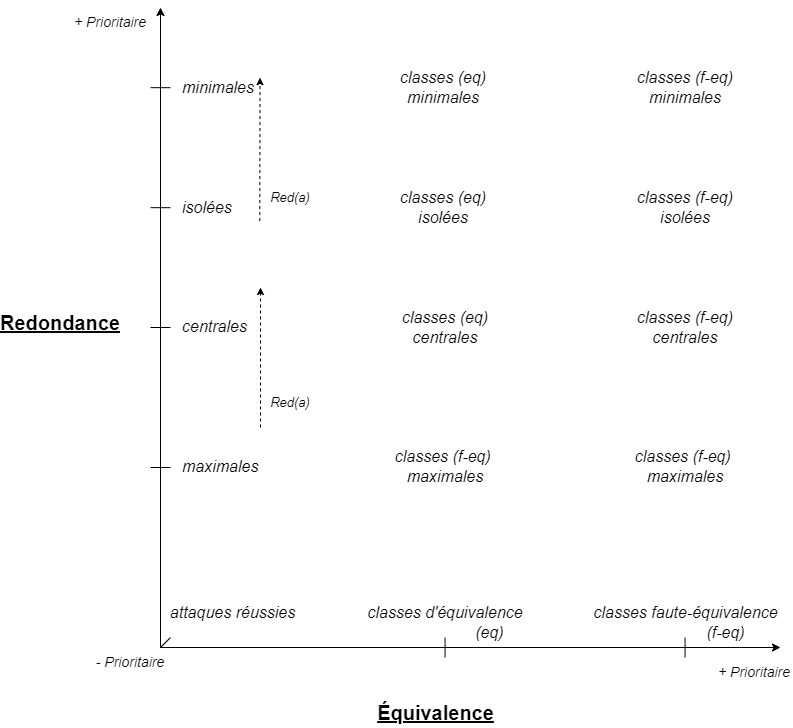
\includegraphics[scale=0.48]{ch3-lazart/img/equiv-redond-priority.png}
                    \caption{Indicatif de priorité des différentes classes d'attaques}  \label{fig:red-eq-priority}
                \end{figure}
            
            \subsubsection{Autres définitions}
            \label{sec:red-otherdef}
            
                Cette section discute des différentes définitions d'équivalence et de redondance proposées par Lazart et des autres définitions qui pourraient être considérées par l'utilisateur.
                
                Les définitions d'équivalence et redondance présentées précédemment ne prennent pas en compte le type de terminaison des traces.
                En effet, on considère que si différents types de terminaison sont considérés comme des attaques par l'utilisateur, alors ces types de terminaison sont équivalents.
                Il est possible de considérer des définitions séparant les attaques en fonction de leur terminaison, par exemple en différenciant les traces terminant en validant l'objectif d'attaque (Satisfy) et les erreurs à l'exécution (\gls{rte})).
                
                Les notions de faute-équivalence et les définitions de redondance considèrent uniquement les fautes, et font donc abstraction des variations de chemins entre les injections de fautes.
                Cette abstraction est très générale, et si un utilisateur souhaite capter \textit{uniquement} des variations liées à l'itération de boucle par exemple, alors il est nécessaire d'utiliser une définition plus spécifique.
                Cela pourrait être implémenté en vérifiant que les transitions non fautées entre deux fautes sur un même point d'injection ne sortent pas d'une boucle par exemple.
                
                Au delà de ces considérations, le concept de redondance pourrait être raffiné. La figure \ref{fig:red-eq-priority} présentée précédemment inclut $Red(a)$ comme paramètre de la priorité des attaques à regarder.
                L'idée est que dans une même classe d'attaques, il peut être intéressant de regarder en priorité les attaques avec $Red(a)$ élevé puisque corriger ces attaques impliquera potentiellement la correction des attaques redondantes dans $Red(a)$.
                Et à l'inverse, les attaques maximales, dans un contexte où l'on souhaite écarter les attaques les moins \og prioritaires \fg{}, pourraient être classées par $Red(a)$ décroissant.
                
                Des définitions se basant sur la relation $Max(a) < Mid(a) < Isol(a) < Min(a)$ pourraient aussi être envisagées.
                Celles-ci pourraient être étendues à des ordres multiples, par exemple: $Max_{n}(a) < Max_{n+1}(a) < ... < Min_n(a) <  Min_{n+1}(a)$ (avec $n$ une limite de faute).
                
                Lazart laisse donc l'utilisateur définir sa propre relation d'ordre partiel, constituée d'une définition d'équivalence et de redondance.
                Par défaut, l'analyse de redondance-équivalence utilise la définition \textit{faute-équivalence} et la redondance en \textit{préfixe}.
          
        \subsection{Analyse de points chauds}
        \label{sec:hotspots}
            
            L'analyse de points chauds (\textit{hotspots}) vise à obtenir des métriques sur les points d'injection sur un ensemble de traces. 
            La section \ref{sec:hs-metrics} présente les métriques proposées par l'analyse de points chauds. 
            La section \ref{sec:hs-redeq} discute de l'exploitation des résultats en fonction de l'ensemble de traces sur lequel l'analyse de points chauds est appliquée.
            
            \subsubsection{Métriques}
            \label{sec:hs-metrics}
            
                L'analyse de points chauds parcourt un ensemble de traces d'exécution et fournit pour chaque point d'injection $i$ et pour chaque nombre de fautes $n$ les données suivantes:
                \begin{itemize}
                    \item \textit{fc}: nombre de traces en $n$ fautes dans lesquelles le point d'injection $i$ est déclenché. 
                    \item \textit{tc}: nombre total de déclenchements de $i$ (en comptant les multiples déclenchements au sein d'une trace).
                    \item \textit{mc}: maximum de déclenchements de $i$ au sein d'une même trace.
                \end{itemize}
                
                Dans le cadre d'aide au placement des contre-mesures dans un programme, \textit{fc} et \textit{tc} permettent d'identifier les points d'injection les plus sensibles à protéger en priorité (voir chapitre \ref{chpt:placement}). 
                Dans le cadre d'une analyse de robustesse, ces deux métriques permettent de déterminer les points d'injection les plus sensibles pour une expertise manuelle ou comme guide pour une analyse plus précise (par exemple une simulation à plus bas niveau).
                Dans un contexte d'heuristiques de sélection de points d'injection (voir section \ref{sec:lazart-metho-andtools}), \textit{mc} permet d'identifier les points d'injection qui sont situés dans des parties répétées du flot de contrôle, et dont le retrait pourrait sensiblement réduire l'explosion combinatoire des fautes.
                De la même façon \textit{tc} (et le ratio \textit{fc}/\textit{tc}) peuvent indiquer qu'un point d'injection a une influence forte sur l'explosion combinatoire des chemins.
            
                La table \ref{tbl:hotspots-results} présente les résultats de l'analyse de points chauds pour le programme \texttt{memcmps} jusqu'à 4 fautes.
                La colonne "IP" indique l'identifiant du point d'injection. 
                La colonne "Info" précise le type de modèle et la ligne correspondant dans le code C (voir listing \ref{lst:example-memcmps}). Les colonnes suivantes indiquent la valeur de $fc$ (nombre de traces déclenchant le point d'injection) pour chaque nombre de faute.
                Les valeurs $tc$ et $mc$ ne sont pas présentées pour cet exemple puisqu'il n'y a pas de trace contenant plusieurs déclenchements d'un même point d'injection\footnote{Cela implique $fc = tc$, $tc > 0 \implies mc = 1$ et $tc = 0 \implies mc = 0$}.
                Dans cet exemple, l'IP 1 est le plus sensible en 1 faute, puisqu'il intervient dans deux attaques.
               
                \begin{table}[htpb]
                    \footnotesize
                    \caption{Résultats d'analyse de points chauds sur \texttt{memcmps}}
                    \label{tbl:hotspots-results}
                    \begin{center}
                        \begin{tabular}{|c|l|c|c|c|c|}
                        \hline
                        IP & \multicolumn{1}{c|}{Info} & 1 faute & 2 fautes & 3 fautes & 4 fautes \\ \hline
                        0 & \begin{tabular}[c]{@{}l@{}}type: ti\\ ligne: 14\end{tabular} & 0 & 1 & 2 & 3 \\ \hline
                        1 & \begin{tabular}[c]{@{}l@{}}type: data\\ ligne: 15\end{tabular} & 0 & 2 & 5 & 7 \\ \hline
                        2 & \begin{tabular}[c]{@{}l@{}}type: ti\\ ligne: 16\end{tabular} & 0 & 0 & 4 & 7 \\ \hline
                        3 & \begin{tabular}[c]{@{}l@{}}type: data\\ ligne: 17\end{tabular} & 0 & 0 & 1 & 3 \\ \hline
                        4 & \begin{tabular}[c]{@{}l@{}}type: ti\\ ligne: 18\end{tabular} & 0 & 0 & 1 & 4 \\ \hline
                        5 & \begin{tabular}[c]{@{}l@{}}type: data\\ ligne: 19\end{tabular} & 0 & 0 & 0 & 1 \\ \hline
                        6 & \begin{tabular}[c]{@{}l@{}}type: data\\ ligne: 24\end{tabular} & 1 & 1 & 2 & 3 \\ \hline
                        \end{tabular}
                    \end{center}
                \end{table}  
            
            \subsubsection{Application sur d'autres ensembles de traces}
            \label{sec:hs-redeq}
            
                Par défaut, l'analyse de points chauds considère toutes les attaques réussies. Il est possible d'appliquer cette analyse sur un ensemble arbitraire de traces et en fonction de l'ensemble de traces sélectionné, les résultats peuvent être interprétés différemment:
            
                \begin{itemize}
                    \item \textit{attaques réussies minimales}: permet de déterminer les \gls{ip}s les plus sensibles (pour expertise manuelle ou afin de placer des protections).
                    \item \textit{attaques réussies}: 
                        \begin{itemize}
                            \item déterminer les \gls{ip}s les plus sensibles sans utiliser la notion de redondance.
                            \item déterminer les \gls{ip}s les plus coûteux pour l'exécution concolique.
                        \end{itemize}
                    \item \textit{attaques réussies maximales}: les \gls{ip}s qui se déclenchent le plus dans des attaques jugées non prioritaires à observer. 
                \end{itemize}
                
                En comparant les résultats obtenus par des analyses de points chauds sur des ensembles de traces différents, il est possible d'obtenir d'autres propriétés:
                \begin{itemize}
                    \item les \gls{ip}s qui se déclenchent dans les attaques maximales mais pas dans les attaques minimales, peuvent ainsi être retirés en priorité d'une analyse en limitant le nombre d'attaques qui ne seraient pas découvertes.
                    \item les \gls{ip}s se déclenchant dans les attaques maximales en sous-mot, mais pas dans les attaques minimales en préfixe, permettent de mettre en évidence des \gls{ip}s qui n'ont pas d'impact, puisqu'ils ne permettent de gagner que si d'autres fautes ont déjà permis de gagner.  
                \end{itemize}
                
                L'analyse de points chauds est donc utile dans différents contextes d'analyse, et le choix de l'ensemble de traces à considérer, voir la comparaison de plusieurs analyses de points chauds, permet d'obtenir des métriques pour des cas d'usage plus précis.
            
    \section{Résultats et méthodologie}
    \label{lazart:metho}
     
        Lazart vise à aider l'utilisateur en traitant les résultats qui lui sont fournis. Les concepts de redondance, d'équivalence et de points chauds présentés précédemment en sont un exemple.
        L'\gls{api} Python vise à rendre la manipulation des résultats plus simple pour l'utilisateur et divers outils, tels que la génération des graphes d'attaques, permettent aussi d'aider à l'interprétation des résultats pour l'utilisateur.
        
        Cependant, certaines problématiques liées à l'utilisation de Lazart se posent.
        Naturellement les limitations dues à KLEE et à l'exécution concolique (voir section \ref{sec:dse}) telles que l'analyse de bibliothèques externes ou l'explosion combinatoire sont héritées par Lazart. 
        La combinatoire des fautes renforce ce problème, d'autant plus en fautes multiples, et les fautes peuvent aussi introduire des chemins qui ne terminent pas (voir section \ref{sec:dse-fi}).
        Le passage à l'échelle peut s'avérer difficile en fonction du code, des modèles de faute et de l'analyse considérés.
        
        La sélection du périmètre de l'analyse est une problématique courante dans l'analyse statique de code, et qui a un impact fort sur le passage à l'échelle: ce périmètre devant parfois être réduit pour permettre que l'analyse termine dans le temps imparti.
        Dans le cadre de l'outil Lazart, ce périmètre correspond au choix de l'objectif d'attaque, du contexte (point d'entrée, entrées du programme), des modèles de faute (et la surface de code sur laquelle ils sont appliqués) et de la surface du programme à analyser.
        
        Enfin, les retours sur la complétude et la correction de l'analyse ne sont pas forcément faciles à interpréter. Il peut être difficile de savoir si les réductions du périmètre de l'analyse n'ont pas pour effet de rater un chemin d'attaque (incomplétude), ou si une concrétisation a eu un effet sur la correction.
        Des précautions concernant le paramétrage de KLEE et de Lazart permettent cependant d'éviter certaines pertes de complétude et de correction.
        
        Le chapitre \ref{chpt:lazart-implem} revient sur l'implémentation de Lazart et discute de ce qui a été fait au niveau de l'outil pour limiter ces problématiques.
        Cette section se concentre sur les résultats et leur exploitation du point de vue de l'utilisateur. 
        La section \ref{sec:lz:exp:results} revient sur les résultats qui sont fournis par l'outil, en présentant une expérimentation réalisée sur un ensemble de programmes, et comment ces résultats peuvent être exploités par l'utilisateur.
        La section \ref{sec:lazart-metho-andtools} s'intéresse à l'aspect méthodologique de l'utilisation de l'outil afin de pallier les différentes problématiques énoncées précédemment.
        Finalement, la section \ref{sec:rsa-strat} discute des autres variables du périmètre d'analyse et présente l'exemple du choix de la stratégie d'exploration dans le cas d'une analyse qui est interrompue avant son terme.        
        
        \subsection{Sorties de l'outil}
        \label{sec:lz:exp:results}
        
            Les métriques sorties par Lazart peuvent être réparties en trois catégories principales:
            \begin{itemize}
                \item Les métriques \textit{statiques}: nombre d'instructions \gls{llvm}, nombre de branchements, nombre de points d'injection, paramètres de l'analyse... % IP, Dets, BRs, Instrs
                \item Les métriques d'\textit{analyse}: nombre d'attaques, nombre d'attaques minimales, métriques de points chauds...
                % Atk, Min, Eq, MinEq
                \item Les métriques d'\textit{exécution}: temps d'exécution, nombre de traces générées, nombre d'instructions exécutées, couverture du code...
                % KTests, Traces, TTotal, TCompile, TDSE, TAnalysis, TLazart, Executed Instructions
            \end{itemize}
            
            La section \ref{sec:lz:exp:bench} présente les différents programmes d'exemples étudiés dans cette section, ainsi que le modèle d'attaquant pour chacun d'entre-eux.
            La section \ref{sec:lz:exp:aar} s'intéresse aux résultats des analyses d'attaques, de redondance, d'équivalence et de points chauds.
            La section \ref{sec:lz:exp:exec} porte sur les métriques d'exécution et de couverture.
            Finalement, la section \ref{sec:lz:exp:cov} s'intéresse à la couverture, la correction et le déterminisme des analyses.
                
            \subsubsection{Ensemble de programmes}
            \label{sec:lz:exp:bench}
            
                Les programmes étudiés ici sont issus de la collection \gls{fissc} 3\footnote{Correspondant à une version enrichie de la collection \gls{fissc} présentée dans \cite{Dureuil/PPLCC16}.} qui est utilisée par Lazart: 
                \begin{itemize}
                    \item $vp$: une collection de \textit{verify\_pin}.
                    \item $rsa$: une collection d'implémentations de l'algorithme \textit{CRT-RSA}.
                    \item $fu$: une collection d'implémentations d'un chargeur de micro-programme.
                \end{itemize}
                
                Les programmes \textit{verify\_pin} sont analysés avec le modèle de l'inversion de test et l'objectif d'attaque de s'authentifier avec un \gls{pin} invalide. 
                La table \ref{tbl:vp-fissc-cms} présente les huit versions étudiées et leurs protections:
                \begin{itemize}
                    \item \textit{HB}: booléens endurcis.
                    \item \textit{FTL}: boucles en temps constant.
                    \item \textit{INL}: inlining de la fonction compare.
                    \item \textit{DTC}: décrémentation anticipée du compteur d'essai \texttt{try\_counter}.
                    \item \textit{TCBK}: duplication du compteur d'essai.
                    \item \textit{CD}: double appel à la fonction \texttt{compare}.
                    \item \textit{TD}: duplication des tests.
                    \item \textit{SC}: compteur d'étape.
                \end{itemize}
                
                \begin{table}[h]
                    \small
                        \caption{Différentes versions de \textit{verify\_pin}}
                        \label{tbl:vp-fissc-cms}
                    \begin{center}
                    \begin{tabular}{ccccccccc}
                    Version & HB & FTL & INL & DTC & TCBK & CD & TD & SC \\
                    \hline
                    vp0 & - & - & - & - & - & - & - & - \\
                    vp1 & \checkmark & - & - & - & - & - & - & - \\
                    vp2 & \checkmark & \checkmark & - & - & - & - & - & - \\
                    vp3 & \checkmark & \checkmark & \checkmark & - & - & - & - & - \\
                    vp4 & \checkmark & \checkmark & - & \checkmark & \checkmark & - & - & - \\
                    vp5 & \checkmark & \checkmark & - & \checkmark & - & \checkmark & - & - \\
                    vp6 & \checkmark & \checkmark & \checkmark & \checkmark & - & - & \checkmark & - \\
                    vp7 & \checkmark & \checkmark & \checkmark & \checkmark & - & - & \checkmark & \checkmark
                    \end{tabular}
                    \end{center}
                \end{table}  
            
                Les expérimentations sur les programmes \gls{rsa} utilisent le modèle de mise-à-0 (\textit{reset}). L'objectif d'attaque correspond à la recherche d'une attaque de type bellcore \cite{boneh2001importance} visant les restes du CRT (recomposition par théorème des restes chinois). 
                Trois versions sont étudiées \cite{puys2014high}:
                \begin{itemize}
                    \item $rsa0$: version non protégée.
                    \item $rsa1$: implémentation de la version Shamir \cite{shamir1999method}.
                    \item $rsa2$: implémentation de la version Aumuller \cite{Aumuller/CHES02}.
                \end{itemize}
                
                \paragraph{}
    
                Deux versions de $fu$ seront étudiées: $fu1$ et $fu2$.
                $fu1$ correspond à la version du programme utilisée dans \cite{Boespflug/FDTC20}, utilisant une duplication de test systématique, et est analysée avec la combinaison du modèle de mutation de données non contrainte (symbolique) et du modèle de l'inversion de test. 
                Les expérimentations se concentrent sur l'objectif d'attaque correspondant à mettre à jour un micro-programme avec un code corrompu ou à ne pas mettre à jour le micro-programme malgré l'intégrité du code d'entrée.
                $fu2$ inclut des protections telles qu'un code détecteur d'erreur dans les pages du micro-programme et des vérifications d'intégrité (voir annexe \ref{annexe:prgm:fu2}).
                Ce programme est analysé avec les modèles \gls{TI} et \gls{DL} séparément\footnote{L'analyse ne termine pas en moins de 12h en combinant les deux modèles.}, les résultats correspondants seront respectivement notés $fu2$ $TI$ et $fu2$ $DL$. L'objectif d'attaque consiste à charger au moins une donnée corrompue (soit une valeur invalide dans le micro-programme, soit l'écriture en dehors de l'espace mémoire du micro-programme).
                
            \subsubsection{Résultats des analyses d'attaque}
            \label{sec:lz:exp:aar}
                
                La table \ref{tbl:ch3:exp:fissc-results} indique les résultats obtenus avec Lazart pour les analyses.
                Pour chaque programme d'exemple (colonne "Nom"), la colonne "LoCs" correspond au nombre de lignes de code du programme étudié\footnote{Cette valeur n'est pas une sortie de l'outil et a été calculée manuellement.}\footnote{En ne prenant pas en compte le code nécessaire à l'analyse (script d'analyse et instrumentation).}, la colonne "IPs" au nombre de points d'injection et la colonne "Det" aux nombre de points de détection des contre-mesures.
                La colonne "Attaques" correspond aux attaques réussies totales pour chaque nombre de fautes tandis que la colonne "Minimales" correspond aux attaques minimales pour une définition en sous-mot.
                Pour chaque ligne, la colonne "Eq" indique l'équivalence des attaques: "atq" correspond aux attaques indépendemment de l'équivalence et "f-eq" correspond aux nombre de classes de faute-équivalence.
                
                \begin{table}[p]
                    \scriptsize
                        \caption{Analyse d'attaque sur le benchmark d'exemple}\label{tbl:ch3:exp:fissc-results}
                    \begin{center}
                        \setlength\tabcolsep{3pt}
                        \begin{tabular}{llll|llllll|lllll|l}
                        \multicolumn{4}{l|}{Programme} & Eq & \multicolumn{5}{l|}{Attaques} & \multicolumn{5}{l|}{Minimales} &  \\
                        Nom & LoCs & IPs & Dets &  & 1F & 2F & 3F & 4F & Total & 1F & 2F & 3F & 4F & Total & TA\% \\
                        \hline
                        \hline
                        vp0 & 25 & 4 & 0 & atq: & 12 & 21 & 18 & 7 & 58 & 12 & 0 & 0 & 0 & 12 & 4 \\
                         &  &  &  & f-eq: & 3 & 3 & 3 & 3 & 12 & 3 & 0 & 0 & 0 & 3 &  \\
                        \hline
                        vp1 & 28 & 5 & 0 & atq: & 12 & 21 & 18 & 7 & 58 & 12 & 0 & 0 & 0 & 12 & 6,5 \\
                         &  &  &  & f-eq: & 3 & 3 & 3 & 3 & 12 & 3 & 0 & 0 & 0 & 3 &  \\
                        \hline
                        vp2 & 39 & 7 & 2 & atq: & 34 & 122 & 204 & 183 & 543 & 34 & 4 & 0 & 0 & 38 & 48 \\
                         &  &  &  & f-eq: & 3 & 4 & 7 & 0 & 14 & 3 & 1 & 0 & 0 & 4 &  \\
                        \hline
                        vp3 & 35 & 7 & 1 & atq: & 34 & 122 & 204 & 183 & 543 & 34 & 4 & 0 & 0 & 38 & 47 \\
                         &  &  &  & f-eq: & 3 & 4 & 7 & 0 & 14 & 3 & 1 & 0 & 0 & 4 &  \\
                        \hline
                        vp4 & 45 & 11 & 6 & atq: & 34 & 118 & 180 & 147 & 479 & 34 & 0 & 4 & 0 & 38 & 41 \\
                         &  &  &  & f-eq: & 3 & 3 & 5 & 7 & 18 & 3 & 0 & 1 & 0 & 4 &  \\
                        \hline
                        vp5 & 37 & 7 & 5 & atq: & 0 & 80 & 644 & 2566 & 3290 & 0 & 80 & 124 & 16 & 220 & 74 \\
                         &  &  &  & f-eq: & 0 & 9 & 20 & 48 & 77 & 0 & 9 & 6 & 1 & 16 &  \\
                        \hline
                        vp6 & 39 & 8 & 6 & atq: & 4 & 40 & 122 & 199 & 365 & 4 & 34 & 0 & 0 & 38 & 10 \\
                         &  &  &  & f-eq: & 1 & 4 & 4 & 7 & 16 & 1 & 3 & 0 & 0 & 4 &  \\
                        \hline
                        vp7 & 78 & 8 & 8 & atq: & 4 & 36 & 116 & 173 & 329 & 4 & 30 & 0 & 0 & 34 & 21 \\
                         &  &  &  & f-eq: & 1 & 3 & 3 & 4 & 11 & 1 & 2 & 0 & 0 & 3 &  \\
                        \hline
                        rsa0 & 65 & 15 & 0 & atq: & 7 & 37 & 151 & 425 & 620 & 7 & 0 & 0 & 0 & 7 & 40 \\
                         &  &  &  & f-eq: & 7 & 37 & 151 & 425 & 620 & 7 & 0 & 0 & 0 & 7 &  \\
                        \hline
                        rsa1 & 92 & 36 & 0 & atq: & 5 & 25 & 118 & 423 & 571 & 5 & 0 & 0 & 0 & 5 & 36 \\
                         &  &  &  & f-eq: & 5 & 25 & 118 & 423 & 571 & 5 & 0 & 0 & 0 & 5 &  \\
                        \hline
                        rsa2 & 109 & 52 & 0 & atq: & 5 & 22 & 106 & 420 & 553 & 5 & 3 & 5 & 19 & 32 & 37 \\
                         &  &  &  & f-eq: & 5 & 22 & 106 & 420 & 553 & 5 & 3 & 5 & 19 & 32 &  \\
                        \hline
                        fu1 & 93 & 23 & 0 & atq: & 1 & 72 & 915 & 8191 & 9179 & 1 & 32 & 915 & 8191 & 9139 & 61 \\
                         &  &  &  & f-eq: & 1 & 8 & 9 & 25 & 43 & 1 & 8 & 9 & 13 & 31 &  \\
                        \hline
                        fu2 TI & 126 & 7 & 0 & atq: & 17 & 119 & 425 & 1031 & 1592 & 17 & 2 & 10 & 53 & 82 & 80 \\
                         &  &  &  & f-eq: & 2 & 3 & 7 & 14 & 26 & 2 & 1 & 2 & 3 & 8 &  \\
                        \hline
                        fu2 DL & 126 & 4 & 0 & atq: & 16 & 344 & 3553 & 23324 & 27237 & 16 & 344 & 1576 & 5624 & 7560 & 52 \\
                         &  &  &  & f-eq: & 1 & 5 & 19 & 67 & 92 & 1 & 5 & 11 & 27 & 44 &  \\
                        \hline
                        \hline
                         & \multicolumn{3}{c|}{\multirow{2}{*}{Moyennes}} & atq: & 13 & 84 & 484 & 2663 & 3244 & 13 & 38 & 188 & 993 & 1233 & \multicolumn{1}{r}{\textbf{39\%}} \\
                         & \multicolumn{3}{c|}{} & f-eq: & 3 & 10 & 33 & 103 & 149 & 3 & 2 & 2 & 5 & 12 &  \\
                         &  &  &  &  &  & \multicolumn{3}{l}{f-eq / atq :} & \multicolumn{1}{r|}{\textbf{4,58\%}} &  & \multicolumn{3}{l}{f-eq / min :} & \multicolumn{1}{r|}{\textbf{0,97\%}} &  \\
                         &  &  &  &  &  & \multicolumn{3}{l}{min / atq :} & \multicolumn{1}{r|}{\textbf{37,9\%}} &  & \multicolumn{3}{l}{min / f-eq :} & \multicolumn{1}{r|}{\textbf{8,08\%}} &  \\
                         &  &  &  &  &  &  &  &  &  &  & \multicolumn{3}{l}{f-eq\_min / atq :} & \multicolumn{1}{r|}{\textbf{0,37\%}} & 
                        \end{tabular}
                    \end{center}
                \end{table} 
            
                \begin{table}[p]
                    \scriptsize
                    \caption{Métriques d'exécution pour le benchmark d'exemple}\label{tbl:ch3:exp:fissc-time}
                    \begin{center}
                    \setlength\tabcolsep{2pt} 
                    \begin{tabular}{l|r|r|r|r|r|r|r|r|r|r|r|r|r}
                    \multicolumn{1}{c|}{\multirow{2}{*}{Nom}} & \multicolumn{1}{c|}{\multirow{2}{*}{EI}} & \multicolumn{5}{c|}{Chemins} & \multicolumn{3}{c|}{Couverture (\%)} & \multicolumn{4}{c}{Temps (s)} \\
                    \multicolumn{1}{c|}{} & \multicolumn{1}{c|}{} & \multicolumn{1}{c}{TR} & \multicolumn{1}{c}{KT} & \multicolumn{1}{c}{CP} & \multicolumn{1}{c}{EP} & \multicolumn{1}{c|}{PP} & \multicolumn{1}{c}{Instrs} & \multicolumn{1}{c}{BBs} & \multicolumn{1}{c|}{BRs} & \multicolumn{1}{c}{DSE} & \multicolumn{1}{c}{TP} & \multicolumn{1}{c}{TA} & \multicolumn{1}{c}{Tot} \\
                    \hline
                    \hline
                    vp0 & 2125 & 9 & 11 & 9 & 17 & 11 & 100 & 100 & 100 & 0.05 & 0.02 & 0.002 & 00.345 \\
                    vp1 & 2647 & 9 & 12 & 9 & 23 & 18 & 97.73 & 100 & 100 & 0.06 & 0.015 & 0.001 & 00.367 \\
                    vp2 & 18085 & 51 & 62 & 51 & 171 & 149 & 97.59 & 100 & 100 & 0.14 & 0.123 & 0.008 & 04.230 \\
                    vp3 & 17855 & 51 & 62 & 51 & 171 & 149 & 97.41 & 100 & 100 & 0.12 & 0.105 & 0.008 & 04.268 \\
                    vp4 & 20259 & 39 & 54 & 39 & 198 & 206 & 96.73 & 100 & 100 & 0.15 & 0.076 & 0.006 & 04.175 \\
                    vp5 & 149490 & 197 & 626 & 197 & 964 & 1781 & 98.25 & 100 & 100 & 0.61 & 0.482 & 0.161 & 01:27 \\
                    vp6 & 17769 & 32 & 55 & 32 & 169 & 172 & 97.86 & 100 & 100 & 0.12 & 0.068 & 0.005 & 03.221 \\
                    vp7 & 25205 & 23 & 34 & 23 & 260 & 328 & 95.57 & 100 & 100 & 0.22 & 0.047 & 0.003 & 04.112 \\
                    rsa0 & 769534 & 621 & 622 & 621 & 673 & 673 & 81.76 & 76.67 & 76.92 & 1.22 & 1.142 & 1.692 & 4.242 \\
                    rsa1 & 421298 & 572 & 573 & 572 & 1597 & 1597 & 56.79 & 50 & 100 & 1.32 & 1.095 & 1.504 & 4.147 \\
                    rsa2 & 507016 & 554 & 557 & 554 & 1104 & 1104 & 55.2 & 47.73 & 75 & 1.26 & 1.032 & 1.505 & 4.079 \\
                    fu 1 & 36632126 & 9179 & 9183 & 9179 & 137670 & 128491 & 97.06 & 91.67 & 85.14 & 08:25 & 31.366 & 13:58 & 22:46 \\
                    fu 2 TI & 1424370 & 1592 & 1597 & 1592 & 2783 & 1191 & 98.51 & 95 & 90 & 4.61 & 3.492 & 34.685 & 43.47 \\
                    fu 2 DL & 15222597 & 27237 & 27240 & 27237 & 59807 & 32570 & 96.97 & 92.5 & 85 & \texttt{1:21:12} & 01:12 & \texttt{1:32:06} & \texttt{2:54:46} \\
                    vp0 sym & 12734 & 58 & 61 & 58 & 130 & 75 & 100 & 100 & 100 & 0.17 & 0.103 & 0.024 & 00.345 \\
                    vp1 sym & 16856 & 58 & 62 & 58 & 178 & 132 & 97.97 & 100 & 100 & 0.19 & 0.106 & 0.024 & 00.367 \\
                    vp2 sym & 190112 & 543 & 633 & 543 & 1930 & 1671 & 97.82 & 100 & 100 & 0.97 & 1.057 & 2.047 & 04.230 \\
                    vp3 sym & 187944 & 543 & 633 & 543 & 1930 & 1671 & 97.67 & 100 & 100 & 0.96 & 1.119 & 2.040 & 04.268 \\
                    vp4 sym & 229512 & 479 & 578 & 479 & 2419 & 2387 & 97 & 100 & 100 & 1.29 & 1.003 & 1.730 & 04.175 \\
                    vp5 sym & 2057305 & 3290 & 9483 & 3290 & 14213 & 24763 & 98.42 & 100 & 100 & 12.61 & 7.189 & 01:05 & 01:27 \\
                    vp6 sym & 188349 & 365 & 547 & 365 & 1941 & 1909 & 98.08 & 100 & 100 & 0.94 & 1.31 & 0.844 & 03.221 \\
                    vp7 sym & 302605 & 329 & 450 & 329 & 3279 & 3954 & 95.88 & 100 & 100 & 1.9 & 1.175 & 0.868 & 04.112
                    \end{tabular}
                    \end{center}
                \end{table} 

                Les pourcentages de réduction des attaques présentées pour l'utilisateur à l'aide de la faute-équivalence et de la redondance sont indiqués en bas de la table.
                On constate qu'en moyenne, la combinaison de la faute-équivalence et de la redondance permet de diviser par un facteur de plus de 100 le total de traces d'attaques à étudier.
                Pour les exemples sur \gls{rsa}, l'analyse de faute-équivalence n'obtient que des groupes d'équivalence d'un élément. Cela peut s'expliquer par l'absence de points d'injection dans les boucles. En revanche, l'analyse de redondance parvient à réduire fortement les attaques, seules les attaques en une faute étant minimales pour $rsa0$ et $rsa1$. 
                
                La colonne "TA\%" indique la part du temps d'exécution de l'analyse qui est consacrée à l'analyse d'équivalence et de redondance. Cette valeur correspond au temps pour la recherche de toutes les relations de redondance et d'équivalences.
                Les analyses d'attaques et de points chauds sont peu coûteuses par rapport à l'analyse de redondance-équivalence qui passe à l'échelle plus difficilement, leurs durées ne sont donc pas présentées ici. 
                En moyenne, l'analyse redondance-équivalence compte pour 39\% du temps d'analyse, mais ce pourcentage varie très fortement d'un programme à l'autre, négligeable dans certains exemples
                mais très coûteux dans d'autres comme vp5.
                Savoir si l'analyse de redondance-équivalence va effectivement réduire de façon significative le nombre d'attaques présentées à l'utilisateur est difficile, puisqu'au delà de la complexité du programme, la structure du graphe de redondance et le nombre de classes d'équivalence peut fortement varier.
            
            \subsubsection{Métriques d'exécution}
            \label{sec:lz:exp:exec}
            
                Un certain nombre de métriques liées à l'exécution de l'analyse sont fournies par Lazart: les métriques de \textit{performance}, les métriques liées aux \textit{chemins} et les métriques de \textit{couverture}.
                
                Les métriques de performance correspondent tout d'abord aux temps d'exécution des différentes étapes de l'analyse: compilation, mutation, exécution concolique, lecture des traces et les différentes traitements.
                KLEE fournit aussi une découpe de son temps d'exécution détaillant la durée de certaines étapes de son exécution (temps de fork, temps d'appel au solveur...) ainsi que des informations concernant l'usage mémoire par exemple.
                
                Les métriques liées aux chemins donnent des informations sur le parcours des chemins dans l'exécution symbolique:
                \begin{itemize}
                    \item Le nombre de ktests générés par KLEE.
                    \item Le nombre de traces générées par Lazart. 
                    \item Le nombre de chemins terminés (\textit{completed paths}), ce qui correspond aux nombre de ktests où l'objectif d'attaque est validé. 
                    \item Le nombre de chemins partiellement explorés (interrompus par un timeout ou une erreur d'exécution par exemple).
                    \item Le nombre de chemins explorés (chemins terminés + chemins partiellement explorés). 
                \end{itemize}
                
                KLEE propose aussi des retours sur la couverture du code: couverture des instructions, des blocs de base et des branchements.
                Lazart calcule également la couverture des points d'injection avec l'analyse de points chauds.
                
                La table \ref{tbl:ch3:exp:fissc-time} présente les résultats obtenus sur l'ensemble des expérimentations.
                Les programmes \texttt{verify\_pin} sont présentés en version avec entrées fixes et symboliques (vpX sym) pour comparaison (la table des résultats d'attaques \ref{tbl:ch3:exp:fissc-results} considère uniquement les versions symboliques).
                La colonne "Nom" correspond au programme et la version considérée.
                La colonne "EI" indique le total d'instructions exécutées par KLEE (au niveau \gls{llvm}).
                Les colonnes "TR" correspond aux nombre de traces générées par Lazart. Pour les paramètres utilisés dans ces exemples, cette valeur est égale au nombre de chemins terminés.
                La colonne "KT" indique le nombre de ktests générés par KLEE.
                Les colonnes "EP" et "PP" correspondent respectivement aux chemins explorés et aux chemins partiellement explorés.
                Les valeurs "EP" et "EI" permettent d'avoir une indication sur la complexité du code étudié.
                
                Les colonnes "Couverture" indiquent dans l'ordre la couverture des instructions ("Instrs"), des blocs de base ("BBs") et des branchements ("BRs") sous la forme de pourcentage.
                La couverture du code sur les programmes \texttt{verify\_pin} est maximale pour les blocs de base et les branches, même dans le cas d'entrées symbolique. La couverture des instructions est la plus précise et donc celle qui fournit les valeurs les plus faibles. Seuls les programmes \gls{rsa} donnent une couverture faible, de l'ordre de 50\% pour les blocs de base et les instructions pour $rsa2$, ce qui peut s'expliquer par le fait que les entrées soient fixées.
                
                Des métriques de temps sont données pour l'exécution symbolique ("DSE"), la lecture des traces ("TP") et pour les différentes analyses ("TA"): analyse d'attaque, analyse de redondance et d'équivalence et analyse de points chauds.
                La durée des étapes de la compilation et de la mutation sont négligeables et ne sont pas mentionnées.
                L'exécution symbolique constitue la part principale des analyses, mais l'analyse de redondance-équivalence peut s'avérer coûteuse dans certains exemples (comme pour vp5 ou fu2).
                
            \subsubsection{Déterminisme, complétude et correction}
                \label{sec:lz:exp:cov}
                
                Cette section s'intéresse au déterminisme des analyses, ainsi qu'aux résultats et métriques fournies par Lazart en ce qui concerne la complétude et la correction d'une analyse (voir définitions section \ref{sec:dse-fi}).
                
                \paragraph{Déterminisme}
                    L'exécution concolique et les solveurs \gls{smt} étant fortement basés sur des heuristiques, qui peuvent inclure de l'aléatoire\footnote{Comme la \textit{random path selection} utilisée par KLEE \cite{Cadar/OSDI08}.}, le déterminisme n'est pas garanti par Lazart.
                    Refaire la même analyse peut donc potentiellement fournir des résultats différents. Les expérimentations réalisées tendent à faire penser que ce non-déterminisme reste relativement rare et davantage présent dans les analyses complexes\footnote{Notez cependant qu'il s'agit là d'un rapport principalement manuel, l'outil ne vérifiant pas le déterminisme automatiquement.}.
                    
                    \paragraph{Couverture et complétude}
                    
                    Lazart effectue une émulation des fautes de telle sorte que l'exploration des chemins et des fautes est complète si l'exécution symbolique explore tous les chemins du mutant.
                    Cependant la complétude peut être perdue à différents niveaux:
                    \begin{itemize}
                        \item au niveau du périmètre de l'analyse et de la configuration de l'outil.
                        \item au niveau de l'exécution concolique elle-même (voir section \ref{sec:dse}: timeout, heuristiques incomplètes).
                        \item []
                    \end{itemize}
                
                    Lazart fournit certaines métriques concernant la complétude, mais cette évaluation reste difficile.
                    Les métriques de couverture fournies par KLEE correspondent à la couverture du programme muté. La couverture des instructions et des blocs de base indiquent donc la couverture du programme original modifié en y incluant le code de simulation des fautes et l'instrumentation de l'analyse.
                    De la même manière, les informations concernant les chemins (EP, PP, CP) présentées précédemment considèrent les chemins du programme muté.
                    
                    Si une couverture incomplète des points d'injection dans le mutant est un signal que la complétude a pu être perdue, une couverture complète des IPs ne veut pas dire que l'analyse est complète.
                    En effet, si deux chemins peuvent déclencher un point d'injection, il suffira qu'un seul des deux soit explorés pour que le point d'injection soit considéré comme couvert. 
                    Lazart tente donc de signaler au maximum les possibles pertes de complétude afin que l'utilisateur puisse estimer la complétude de l'analyse.
                    Lazart indique aussi d'autres métriques telles que les analyses qui ont été interrompues par l'utilisateur ou bien les traces qui n'ont pas pu être rejouées pour cause de timeout\footnote{Notez qu'un ktest peut avoir le type de terminaison différent de \textit{timeout} (le chemin étant terminé du côté de l'exécution symbolique) sans pouvoir être rejoué dans une limite de temps imparti.}, qui constituent une autre indication concernant la complétude.
                    
                    Cependant, si aucune des métriques ne montre une perte de complétude, seule une validation manuelle permet d'avoir des garanties sur le fait que toutes les exécutions fautées ont effectivement été explorées.
                
                    \paragraph{Correction}
                    
                    La correction est une propriété plus délicate puisque très peu de retours sont fournis par KLEE et Lazart.
                    Si l'exécution symbolique classique est \textit{correcte}, l'exécution concolique peut être incorrecte en raison de certaines concrétisations ne préservant pas la correction.
                    
                    KLEE peut donner des informations sur des concrétisations incorrectes, par exemple via la terminaison de traces de type "model". Cela étant, la validation d'un chemin d'attaque par l'utilisateur reste nécessaire.  
            
        \subsection{Méthodologie et chaîne d'outils}
        \label{sec:lazart-metho-andtools}
        
            Cette section s'intéresse à l'aspect méthodologique de l'utilisation de Lazart vis-à-vis des problématique présentées en début de section \ref{lazart:metho}: passage à l'échelle, spécification du périmètre d'analyse et les pertes de complétude.
            
            La méthodologie proposée dans \cite{lacombe2021combining, lacombe2023combining} sera prise pour exemple pour discuter des solutions et approches existantes pour limiter ces problématiques.
            Cette méthodologie vise à limiter la combinatoire des fautes en réduisant le nombre de points d'injection de fautes dans l'analyse.
            Cette approche peut être vue comme une instance particulière d'une méthodologie reposant sur trois grands principes:
            \begin{itemize}
               \item la réduction du périmètre d'analyse par sur-approximation.
               \item l'utilisation d'une chaîne d'outils combinant différentes techniques d'analyse.
               \item une approche itérative par raffinement du périmètre à l'aide d'heuristiques.
            \end{itemize}
            
            Des expérimentations ont été conduites sur les programmes $vp6$ et $vp9$ (voir section \ref{sec:lz:exp:bench}), la commande sudo (de Linux-PAM) et la bibliothèque iso7816 du projet Wookey \cite{wookey}. 
            Ces expérimentations utilisent le modèle XOR (présenté dans le chapitre \ref{chpt:background}) consistant à fauter les expressions au niveau CIL en effectuant une opération XOR avec une donnée fautée. 
            
            La section \ref{sec:lazart:metho:arch} présente la méthodologie proposée.
            La section \ref{sec:lazart:metho:eva} s'intéresse à l'analyse de dépendance,
            les sections \ref{sec:lazart:metho:static} et  \ref{sec:lazart:metho:iter} aux heuristiques qui peuvent être appliquées pour réduire davantage l'ensemble des points d'injection à analyser.
           
            \subsubsection{Présentation générale}
            \label{sec:lazart:metho:arch}
            
                \begin{figure}[!htp]\centering
                    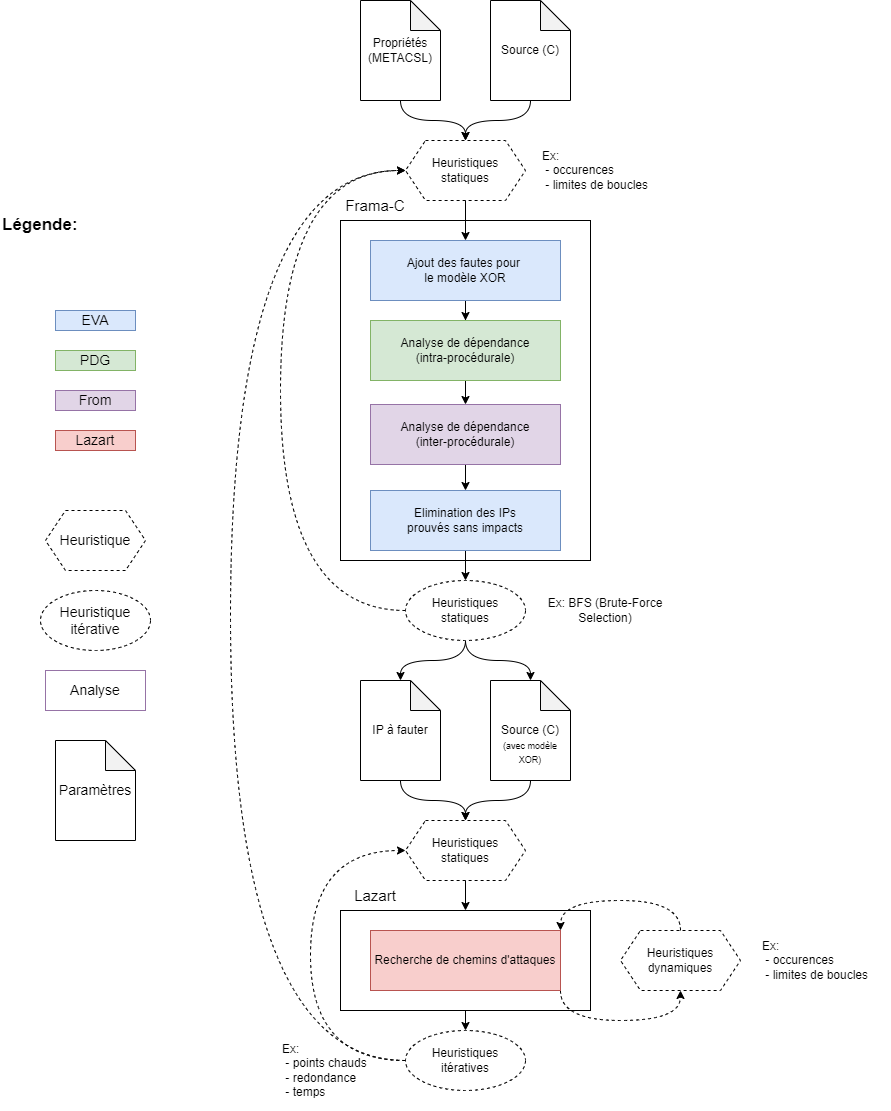
\includegraphics[scale=0.41]{ch3-lazart/img/fdep.drawio.png}
                    \caption{Schéma général de la méthodologie \cite{lacombe2023combining}} \label{fig:metho-fdep}
                \end{figure}
        
                La figure \ref{fig:metho-fdep} présente l'architecture générale de la méthodologie proposée.
                Cette méthodologie utilise l'analyse statique afin de déterminer quels sont les points d'injection qui ont un impact sur la propriété de sécurité étudiée.
                Cet ensemble de fautes est ensuite transmis à Lazart qui recherche des chemins d'attaques.
                Cette approche est présentée dans la section \ref{sec:lazart:metho:eva}.
                Des heuristiques ont aussi été proposées afin de réduire encore l'espace des fautes à injecter. Ces heuristiques peuvent être séparées en deux groupes:
                \begin{itemize}
                    \item Les heuristiques \textit{simples} qui s'appuient sur les résultats d'une unique exécution d'une analyse (section \ref{sec:lazart:metho:static}).
                    \item Les heuristiques \textit{itératives}, qui utilisent une approche itérative pour raffiner le périmètre d'analyse à chaque appel d'un outil, présentées dans la section \ref{sec:lazart:metho:iter}.
                \end{itemize}
                
            \subsubsection{Approximation des points d'injection de fautes utiles}
            \label{sec:lazart:metho:eva}
            
                Cette étape prend en entrée le programme source C et les propriétés à vérifier sous la forme d'assertions (\gls{acsl}). Celles-ci peuvent être définies par l'utilisateur, ou générées automatiquement: les expérimentations conduites utilisent le plugin \gls{rte} de Frama-C permettant de placer automatiquement des assertions contre les erreurs d'exécution.
            
                L'étape d'analyse statique se déroule en quatre sous-étapes:
                \begin{itemize}
                    \item 1) Simulation des points d'injection avec le modèle XOR en introduisant une variable non initialisée (déclarée comme \texttt{extern}) par point d'injection. Cette étape est effectuée avec \gls{eva} qui utilise l'interprétation abstraite (et fonctionne donc par sur-approximation).
                    \item 2) Génération des graphes de dépendances intra-procédural, à l'aide du plugin \gls{pdg} de Frama-C (basé sur \gls{eva}).
                    \item 3) Calcul du graphe de dépendances inter-procédural à l'aide du plugin From.
                    \item 4) Calcul de dépendances pour déterminer quels points d'injection peuvent impacter chaque assertion.
                \end{itemize}
                
                Ainsi, on ne conserve que les points d'injection qui ont un impact (d'après l'analyse de dépendance) sur les assertions non prouvées par \gls{eva}.
                Cette réduction de l'espace de faute préserve la complétude puisque celle-ci est effectuée en considérant toutes les fautes possibles.
                
                La table \ref{tbl:results-fdep} contient les résultats obtenus pour nos programmes de test. La colonne "Nom" indique le programme en question, "IPs" le nombre de points d'injection dans le programme et "Dets" le nombre de points de vérification de contre-mesure (déclenchant un arrêt de la carte si une attaque est détectée).
                La colonne "Lazart (seul)" indique le nombre d'attaques totales trouvées "AP", le nombre de chemins explorés ("EP") et la durée de l'analyse dans le cas où Lazart est lancé sur toutes les fautes générées par le modèle XOR.
                La colonne "AS" correspond à l'étape d'analyse statique (dépendances des propriétés) indiquant le temps d'exécution ("Temps") et le nombre de points d'injection restant après l'analyse ("IPs").
                La colonne Heuristiques indique les heuristiques appliquées ("Type"), le temps d'exécution ("Temps") et le nombre de points d'injection restant après l'application de ces heuristiques ("IPs").
                Enfin, la colonne "Lazart" présente les résultats obtenus avec les points d'injection restants.
                
                Les programmes "vp0" et "vp7" ont été testés sans heuristique (les valeurs \mbox{"-"} indiquant qu'une étape n'est pas effectuée) et permettent d'illustrer un gain de temps non négligeable avec cette analyse de dépendance préliminaire. L'interprétation abstraite passe communément mieux à l'échelle et c'est pourquoi le temps d'analyse reste inférieur à une seconde pour ces exemples.
                Le gain est ainsi bien supérieur pour l'exemple "vp7" qui réduit d'un facteur 10 le nombre de points d'injection à analyser pour Lazart, pour un temps d'analyse trois fois moindre.
                
                \begin{table}[!htpb]
                    \scriptsize
                        \caption{Résultats obtenus pour l'analyse de dépendance}\label{tbl:results-fdep}
                    \begin{center}
                        \setlength\tabcolsep{4pt}
                        \begin{tabular}{l|c|c|c|c|c|c|c|c|c|c|c|c|c}
                        \multicolumn{3}{l|}{Programme} & \multicolumn{3}{l|}{Lazart (seul)} & \multicolumn{2}{l|}{AS} & \multicolumn{3}{l|}{Heuristique} & \multicolumn{3}{l}{Lazart} \\
                        \hline
                        \multicolumn{1}{l|}{Nom} & \multicolumn{1}{l}{IPs} & \multicolumn{1}{l|}{Dets.} & \multicolumn{1}{l|}{AP} & \multicolumn{1}{l|}{EP} & \multicolumn{1}{l|}{Temps} & \multicolumn{1}{l|}{Temps} & \multicolumn{1}{l|}{IPs} & \multicolumn{1}{l|}{Type} & \multicolumn{1}{l|}{Temps} & \multicolumn{1}{l|}{IPs} & \multicolumn{1}{l|}{Attaques} & \multicolumn{1}{l|}{EP} & \multicolumn{1}{l}{Time} \\
                        \hline
                        \hline
                        \multicolumn{1}{l}{vp0} & 20 & 0 & 5 & 65 & \textbf{14s} & 1s & 10 & - & - & - & 5 & 52 & \textbf{11s} \\
                        \multicolumn{1}{l}{vp7} & 142 & 31 & 6 & 3253 & \textbf{1h43} & 1s & 15 & - & - & - & 6 & 1051 & \textbf{30min}
                        \end{tabular}
                    \end{center}
                \end{table} 
                 
            \subsubsection{Heuristiques simples}
            \label{sec:lazart:metho:static}
            
                La méthodologie \cite{lacombe2023combining} propose une heuristique de sélection basée sur le nombre maximal d'occurrences des points d'injection dans une exécution nominale (sans injection de faute).
                Cette heuristique est implémentée avec \gls{eva}, en amont de l'analyse statique de dépendance.
                Cette heuristique fait la supposition qu'un point d'injection qui se déclenche souvent en l'absence de faute, a plus de risque de provoquer une explosion combinatoire des chemins fautés et donc la non-terminaison de l'exploration concolique. 
                Cette heuristique n'est valable qu'en faute unique puisque dans un contexte de fautes multiples, les occurrences des points d'injection peuvent fortement varier.
                
                Une autre heuristique consiste à instrumenter le programme de manière à limiter l'exploration des exécutions.
                Lazart propose des macros d'instrumentation qui coupent l'exploration une fois qu'une limite fixée a été atteinte (par exemple pour limiter les itérations d'une boucle). 
                Lazart n'a cependant pas de solution directe pour définir des limites de fautes différentes pour certains modèles de faute (seule une limite globale de fautes peut être définie). Cela permettrait de limiter l'occurrence de certains points d'injection sans pour autant les ignorer complètement, afin de ne pas passer à côté d'attaques combinées les impliquant. 

                La sélection par force brute (\gls{bfs}) est une heuristique qui a été proposée dans \cite{lacombe2021combining} et qui nécessite plusieurs appels à l'analyseur statique.
                \gls{bfs} consiste à tester indépendamment si un point d'injection a un impact sur les propriétés, en désactivant tous les autres \gls{ip}s. Les points d'injection qui n'ont pas d'impact sur les propriétés sont retirés.
                Cependant, cette approche n'est valide que dans un contexte de faute unique puisque chaque point d'injection est testé indépendamment. Une version multi-fautes nécessiterait d'effectuer autant de fois l'analyse qu'il existe de combinaisons de fautes possibles, ce qui revient à décaler la problématique de l'explosion combinatoire des fautes sur l'analyse de dépendances plutôt que sur l'exécution symbolique.
                La table \ref{tbl:results-fdep2} indique les résultats obtenus avec l'heuristique \gls{bfs} pour l'exemple \textit{iso7816} où près de 60\% des points d'injection peuvent être retirés, en faute unique.
                
            \subsubsection{Heuristiques itératives}
            \label{sec:lazart:metho:iter}
            
                Les heuristiques itératives consistent à raffiner l'espace de faute à injecter au fur et à mesure des analyses. Celles-ci peuvent utiliser l'approche:
                \begin{itemize}
                    \item par \textit{élargissement du périmètre d'analyse}: le périmètre est étendu à chaque itération.
                    \item par \textit{réduction du périmètre d'analyse}: le périmètre est réduit à chaque itération.
                    \item par \textit{combinaison} de réductions et d'élargissement.
                \end{itemize}
                
                Nous avons ainsi proposé une approche par réduction appelée \gls{ss} qui consiste à
                interrompre l'analyse après un temps donné et retirer les points d'injection qui sont les plus déclenchés.
                D'autres métriques produites par l'analyse de points chauds pourraient être considérées pour déterminer les points d'injection à retirer, comme par exemple enlever les points d'injection qui se déclenchent plusieurs fois par attaque (cela étant principalement lié aux boucles).
                Si l'analyse est interrompue mais produit tout de même des attaques, il est possible de retirer les points d'injection apparaissant le plus dans les attaques maximales, puisqu'il s'agit à priori des attaques les moins intéressantes à explorer. 
                Cependant, ces approches par réduction nécessitent de déterminer la durée de seuil du timeout, ce qui n'est pas évident. 
                Dans les cas où seuls quelques points d'injection sont problématiques, ce type d'heuristiques peut fortement aider l'analyse.
                
                L'approche par élargissement que nous avons proposée, appelée \gls{sw}, vise à répéter l'analyse avec Lazart en ajoutant les points d'injection un par un. Si l'analyse dépasse le timeout spécifié lorsqu'un ajoute un point d'injection, alors celui-ci est retiré et un autre point d'injection est testé.
                Il est nécessaire de prévoir une marge par rapport à la durée de l'itération précédente puisque l'ajout d'un point d'injection va nécessairement augmenter le nombre de chemins. Celle-ci a été fixée à 150\% dans nos expérimentations. 
                
                La table \ref{tbl:results-fdep2} présente les résultats obtenus pour les exemples \textit{iso7816} et \textit{sudo}.
                L'exemple sudo a été testé avec la limite des occurrences de points d'injection (réduction) fixée à 1 ("O1") et à 5 ("O5"), et avec l'approche "SW" (élargissement).
                iso7816 a été expérimenté en faute unique avec \gls{bfs} et \gls{sw}, combinée à l'analyse de dépendances (section \ref{sec:lazart:metho:eva}).
                L'approche \gls{bfs}, qui utilise ici un timeout, est très performante car elle réduit très fortement le nombre de points d'injection.
                
                \begin{table}[!htpb]
                \scriptsize
                    \caption{Résultats obtenus pour la méthodologie}\label{tbl:results-fdep2}
                \begin{center}
                    \setlength\tabcolsep{4pt}
                    \begin{tabular}{l|c|c|c|c|c|c|c|c|c|c|c|c}
                    \multicolumn{2}{l|}{Programme} & \multicolumn{3}{l|}{Lazart (seul)} & \multicolumn{2}{l|}{AS} & \multicolumn{3}{l|}{Heuristique} & \multicolumn{3}{l}{Lazart} \\
                    \hline
                    \multicolumn{1}{l|}{Nom} & \multicolumn{1}{l|}{IPs}  & \multicolumn{1}{l|}{AP} & \multicolumn{1}{l|}{EP} & \multicolumn{1}{l|}{Temps} & \multicolumn{1}{l|}{Temps} & \multicolumn{1}{l|}{IPs} & \multicolumn{1}{l|}{Type} & \multicolumn{1}{l|}{Temps} & \multicolumn{1}{l|}{IPs} & \multicolumn{1}{l|}{Attaques} & \multicolumn{1}{l|}{EP} & \multicolumn{1}{l}{Time} \\
                    \hline
                    \hline
                    \multirow{4}{*}{sudo} & 919  & 17 & 737 & 11 & N/A & N/A & \gls{sw} & 23min & 913 & 17 & 737 & 11s \\
                     & 919  & 17 & 737 & 11s & 1s & 104 & \gls{sw} & 3min & 102 & 17 & 670 & 11s \\
                     & 919  & 17 & 737 & 11s & - & - & \gls{sw}+O1 & 3min & 40 & 10 & 602 & 10s \\
                     & 919  & 17 & 737 & 11s & 1s & 104 & \gls{sw}+O5 & 4min & 47 & 10 & 302 & 10s \\
                    \hline
                    \multirow{3}{*}{iso7816} & 153  & - & - & - & -& - & \gls{sw} & 16min & $660 \to 655$  & 1 & 192 & 19s \\
                     & 153  & - & - & - & 153 & 3s & \gls{sw} & 6min  & $153 \to 151$  & 1  & 170 & 12s \\
                     & 153  & - & - & - & 1 & 55s & \gls{bfs} & - & - & 1 & 45 &  1s\\
                    \end{tabular}
                \end{center}
            \end{table} 
        
        \subsection{Périmètre d'analyse de Lazart et analyse partielle}
        \label{sec:rsa-strat}
        
            La méthodologie présentée dans \cite{lacombe2023combining} se concentre sur la sélection des points d'injection sur lesquels une faute pourra être injectée.
            Le modèle XOR englobant la combinaison des modèles d'inversion de test et de données symboliques non contraintes, celui-ci décale la problématique de la sélection des modèles de faute à appliquer vers la problématique de la sélection des points d'injection à activer.
            Comme cela a été évoqué précédemment, le périmètre d'analyse de Lazart inclut aussi d'autres paramètres, notamment le choix de l'objectif d'attaque ou encore de la surface de code à analyser.
            
            Le choix du périmètre d'analyse initial reste une difficulté pour l'utilisateur de l'outil et par exemple, les centres d'évaluation s'appuient en grande partie sur l'expertise des évaluateurs.
            Des méthodes telles que les \textit{stubs}\footnote{Le stub consiste à émuler l'effet d'une partie du programme. Par exemple en remplaçant le corps d'une fonction par un simple retour d'une valeur. Dans ce cas, l'opération est incomplète mais il est possible de préserver la complétude en retournant une variable symbolique dans le cas de Lazart, ce qui revient à faire une sur-approximation des comportements.} peuvent être utilisées pour aider à sélectionner les portions du programme à analyser. L'état de l'art des attaques en fautes permet d'aider à choisir les objectifs d'attaque et modèles de faute à étudier.
            Certains outils d'analyse non liés à l'analyse de fautes peuvent aider à la définition du périmètre d'analyse pour Lazart. Par exemple, l'analyse de dépendances d'\gls{eva} peut permettre ainsi de déterminer quelles fonctions du programme ciblé ont un impact sur les propriétés étudiées et de réduire l'analyse à cette portion.
            Lancer KLEE sur le programme sans injecter de faute (hors de Lazart donc) permet de déterminer si certaines portions du programme posent d'ores et déjà problème pour l'exécution concolique alors qu'aucune faute n'est injectée.
            
            Lorsqu'une analyse est trop complexe pour terminer dans un temps imparti, il est néanmoins possible de récupérer des chemins d'attaques en laissant l'exécution symbolique s'exécuter avec un timeout.
            Dans ce cas, le choix de la stratégie d'exploration est d'autant plus importante que celle-ci peut fortement influer sur les chemins d'attaques qui seront trouvés dans le temps imparti.
            La suite de cette section présente un cas d'utilisation d'une exécution concolique interrompue avec le programme \gls{rsa}.  
           
            Les programmes \gls{rsa} (du \gls{fissc}) n'utilisent pas d'entrées symboliques et utilisent un modèle de mise-à-0 plutôt que la mutation de données symbolique.
            Ces programmes implémentent des opérations modulaires, ce qui implique des boucles dont le nombre d'itérations dépend des entrées.
            Si les entrées ou la valeur d'une faute injectée sont symboliques, alors beaucoup de chemins peuvent être explorés, et potentiellement de longueurs élevées. 
            Néanmoins, il est possible de borner la durée de l'exécution symbolique afin d'obtenir des chemins d'attaques.
            
            La table \ref{tbl:ch3:exp:rsa-strat} présente les résultats obtenus pour le programme d'exemple $rsa0$ avec le modèle d'injection de données en fonction de la stratégie d'exploration utilisée (colonne "Stratégie"). Par défaut, KLEE utilise la stratégie \texttt{nurs-cn} (Non-Uniform Random Search - Coverage-New), visant en priorité les chemins allant vers les instructions les moins couvertes. Les stratégies de recherche en profondeur (\gls{dfs}) et recherche en largeur (\gls{bfs2}) sont également présentées.
            Les colonnes suivantes indiquent le nombre d'attaque réussies trouvées pour chaque nombre de fautes.
            La colonne "EP" correspond au chemins explorés et la colonne "EI" au nombre d'instructions exécutées.
            La colonne "BCov" correspond à la couverture des blocs de base.
            La colonne "TDSE" indique combien de temps l'exécution symbolique a duré\footnote{Le timeout est fixé à 30 minutes mais un temps supplémentaire est nécessaire à KLEE pour générer les ktests correspondant aux chemins en cours d'exploration.}.
            
            \begin{table}[ht]
                \small
                    \caption{Comparaison de différentes stratégies d'exploration}\label{tbl:ch3:exp:rsa-strat}
                \begin{center}
                \setlength\tabcolsep{4pt}
                \begin{tabular}{l|llll|llll}
                Stratégie &1F & 2F & 3F & 4F & EP & EI & BCov & TDSE \\
                \hline
                nurs-cn &  0 & 0 & 0 & 0 & - & - & - & - \\
                dfs &  54 & 71 & 100 & 75 & 419 & 3561393 & 96.8 & 33:37 \\
                bfs &  17 & 18 & 5 & 0 & 95 & 126315 & 33.62 & 57:34:00 \\
                \end{tabular}
                \end{center}
            \end{table} 
            
            On constate que la stratégie d'exploration a un fort impact sur les résultats qui sont obtenus. La stratégie par défaut ne parvient pas à trouver d'attaque en 30 minutes, mais les deux autres stratégies y parviennent, \gls{dfs} trouvant le plus d'attaques dans ce cas. 
            Pour \texttt{nurs-cn}, KLEE ne parvient pas à produire les ktests dans un temps imparti\footnote{Une limite de 1h pour l'arrêt de KLEE a été fixée, mais KLEE ne parvient pas à générer les cas de tests dans le temps imparti et ainsi aucune métrique d'exécution n'est disponible.}.
        
            La table \ref{tbl:ch3:exp:rsa-time} présente les résultats obtenus pour $rsa0$ avec mutation de données symbolique en fonction du temps d'analyse, en utilisant la stratégie d'exploration \gls{dfs}. 
            La colonne "Délai" indique le temps accordé à l'exécution concolique pour l'analyse.
            Les autres colonnes ont la même signification que précédemment (table \ref{tbl:ch3:exp:rsa-strat}). 
            Comme attendu, plus la durée limite est longue, plus l'analyse trouve de chemins d'attaque et plus la couverture est élevée.
            Cela étant, on peut observer que le passage de 1 minute à 5 minutes n'apporte que peu de nouveaux chemins d'attaques (4) tandis que le passage à 30 minutes en ajoute beaucoup.
    
            \begin{table}[ht]
                \small
                    \caption{Attaques trouvées sur RSA en fonction du délai d'analyse spécifié}\label{tbl:ch3:exp:rsa-time}
                \begin{center}
                \setlength\tabcolsep{4pt} 
                    \begin{tabular}{l|llll|lll|l}
                    Délai & 1F & 2F & 3F & 4F & Chemins & Instrs. & BCov & TDSE \\
                    \hline
                    10s & 10 & 5 & 0 & 0 & 35 & 306596 & 90.62 & 00:11 \\
                    1min & 25 & 50 & 50 & 24 & 42 & 1962377 & 93.75 & 01:00 \\
                    5min & 28 & 50 & 50 & 25 & 223 & 1965419 & 96.8 & 05:01 \\
                    30min & 54 & 71 & 100 & 75 & 419 & 3561393 & 96.8 & 33:37
                    \end{tabular}
                \end{center}
            \end{table} 
            
            Le choix de la stratégie d'exploration est un paramètre important pour Lazart, et dans le cas d'analyses qui ne terminent pas en un temps raisonnable, l'utilisation d'un timeout et d'une stratégie d'exploration adaptée permet de tout de même obtenir des résultats. 
            La stratégie d'exploration peut aussi avoir un impact sur la consommation mémoire en fonction du nombre d'états symboliques explorés simultanément.
            Enfin, la stratégie d'exploration est aussi importante dans le cas où l'analyse termine, certaines stratégies pouvant rater des chemins, notamment lorsqu'elle incluent de l'aléatoire.
            
    \section{Conclusion}
        \label{sec:lazart:metho:concl}
        
        La section \ref{lazart:metho} a présenté des solutions et méthodologies permettant de pallier les problématiques liées à l'utilisation de Lazart, notamment en ce qui concerne la sélection des points d'injection à évaluer.
        L'analyse statique permet de réduire l'espace de faute de Lazart de façon considérable sur certains exemples.
        La table \ref{tbl:metho-conclusion} compare certaines des heuristiques présentées précédemment, leur nom étant indiqué dans la première colonne.
        La colonne "Type" détermine si l'heuristique est simple ou itérative. La colonne "Niveau" précise si l'heuristique est appliquée au niveau de l'analyse statique ou de Lazart.
        La colonne "Contexte de fautes" indique si l'heuristique est destinée à la faute unique ou aux fautes multiples et finalement la colonne "Complétude" précise si l'heuristique préserve la complétude.
        
        \begin{table}[hbt]
        \centering
        \caption{Comparaison de différentes heuristiques}
        \vspace{0.2cm}
        {\small
        \label{tbl:metho-conclusion}
            \begin{tabular}{l||l|l|l|l}
            Heuristique & Type & Niveau & Contexte de fautes & Complétude \\
            \hline
            \hline
            Limite d'occurence & simple & \begin{tabular}[c]{@{}l@{}}statique\\ dynamique\end{tabular} & \begin{tabular}[c]{@{}l@{}}simple\\ multiple\end{tabular} & Non \\
            \hline
            Selection bruteforce & iter & statique & simple & Oui \\
            Strategy shrinking & iter & dynamique & simple & Non \\
            Strategy widening & iter & dynamique & multiple & Non \\
            \hline
            Analyse manuelle & both & both & multiple & Non \\ 
            Analyse partielle & both & dynamique & multiple & Non 
        \end{tabular}
        }
        \end{table}
        
        Lazart propose donc des traitements des résultats visant à aider l'utilisateur dans la recherche de vulnérabilité et la protection du programme. 
        Si la définition du périmètre initial d'une analyse reste délicate, l'approche itérative et l'utilisation d'analyse par sur-approximation permettent de guider l'utilisateur.
        
        Le chapitre suivant revient sur ces problématiques du point de vue de l'implémentation. Elle précise certains choix qui ont été faits et qui résultent souvent d'un compromis entre accessibilité, passage à l'échelle et complétude. 
        